\documentclass[aspectratio=169,11pt]{beamer}
% ==========================================================================
%  KSA lecture-slide theme  =  stock beamer "Boadilla"  +  KSA colour theme
%  brand colours sampled from the official KSA symbol mark:
%    Deep Prussian Blue  #2E3192   (지성 - intellect)
%    Golden Gray         #D6CBB1   (감성 - sensibility)
%  Engine: XeLaTeX.  Usage:
%    \documentclass[aspectratio=169,11pt]{beamer}
%    % ==========================================================================
%  KSA lecture-slide theme  =  stock beamer "Boadilla"  +  KSA colour theme
%  brand colours sampled from the official KSA symbol mark:
%    Deep Prussian Blue  #2E3192   (지성 - intellect)
%    Golden Gray         #D6CBB1   (감성 - sensibility)
%  Engine: XeLaTeX.  Usage:
%    \documentclass[aspectratio=169,11pt]{beamer}
%    % ==========================================================================
%  KSA lecture-slide theme  =  stock beamer "Boadilla"  +  KSA colour theme
%  brand colours sampled from the official KSA symbol mark:
%    Deep Prussian Blue  #2E3192   (지성 - intellect)
%    Golden Gray         #D6CBB1   (감성 - sensibility)
%  Engine: XeLaTeX.  Usage:
%    \documentclass[aspectratio=169,11pt]{beamer}
%    \input{../theme/ksa-theme.tex}
% ==========================================================================

\usepackage{fontspec}
\usepackage{amsmath,amssymb}
\usepackage{graphicx}
\graphicspath{{figs/}{../figs/}}
\usepackage{booktabs}
\usepackage{listings}

% ---- fonts (no ctex/xeCJK on this box -> fontspec drives CJK directly) -----
\defaultfontfeatures{Ligatures=TeX}
\setmainfont{Noto Sans CJK KR}
\setsansfont{Noto Sans CJK KR}
\setmonofont{Noto Sans Mono CJK KR}[Scale=0.92]

% ---- base theme: stock Boadilla ------------------------------------------
\usetheme{Boadilla}
\usefonttheme{professionalfonts}
\setbeamertemplate{navigation symbols}{}

% ---- KSA colour theme (recolour the stock theme) --------------------------
\definecolor{ksablue}{HTML}{2E3192}
\definecolor{ksabluedk}{HTML}{20226A}
\definecolor{ksagold}{HTML}{D6CBB1}
\definecolor{ksagolddk}{HTML}{A9976B}
\definecolor{ksared}{HTML}{C0392B}
\definecolor{ksagray}{HTML}{5B5B5B}

\setbeamercolor{structure}{fg=ksablue}
\setbeamercolor{alerted text}{fg=ksared}

\setbeamercolor{palette primary}{fg=white,           bg=ksablue}
\setbeamercolor{palette secondary}{fg=white,         bg=ksablue!85!black}
\setbeamercolor{palette tertiary}{fg=white,          bg=ksabluedk}
\setbeamercolor{titlelike}{fg=ksablue}
\setbeamercolor{frametitle}{fg=ksablue,bg=}
\setbeamercolor{title}{fg=ksablue}
\setbeamercolor{author}{fg=ksagray}
\setbeamercolor{institute}{fg=ksagray}
\setbeamercolor{block title}{fg=white,bg=ksablue}
\setbeamercolor{block body}{fg=black!85,bg=ksablue!6}
\setbeamercolor{item}{fg=ksablue}
\setbeamercolor{section in toc}{fg=black!85}

\setbeamerfont{frametitle}{series=\bfseries}
\setbeamerfont{title}{series=\bfseries}

% ---- footline:  KSA mark | "Made by ..." | n / N   (matches reference) ----
\newcommand{\ksacredit}{Made by Sumin Han \,\textperiodcentered\, suminhan@ksa.hs.kr}
\setbeamertemplate{footline}{%
  \hbox{%
    \begin{beamercolorbox}[wd=.18\paperwidth,ht=2.6ex,dp=1.5ex,leftskip=1.1em]{}%
      \raisebox{-0.35ex}{
\includegraphics[height=2.0ex]{ksa-logo.png}}%
    \end{beamercolorbox}%
    \begin{beamercolorbox}[wd=.64\paperwidth,ht=2.6ex,dp=1.5ex,center]{}%
      {\scriptsize\color{ksagray}\ksacredit}%
    \end{beamercolorbox}%
    \begin{beamercolorbox}[wd=.18\paperwidth,ht=2.6ex,dp=1.5ex,rightskip=1.1em]{}%
      \hfill{\scriptsize\color{ksablue}\insertframenumber\,/\,\inserttotalframenumber}%
    \end{beamercolorbox}%
  }%
  \vskip2pt
}

% ---- section divider: stock \sectionpage, KSA-coloured -------------------
\setbeamertemplate{section page}{%
  \begingroup\centering
    {\color{ksagolddk}\rule{0.16\paperwidth}{1pt}}\par\vskip1.0em
    {\usebeamerfont{title}\color{ksablue}\insertsectionhead\par}\vskip1.0em
    {\color{ksagolddk}\rule{0.16\paperwidth}{1pt}}\par
  \endgroup
}
\AtBeginSection[]{\begin{frame}[plain,noframenumbering]\vfill\sectionpage\vfill\end{frame}}

% ---- code listings ------------------------------------------------------------
\lstdefinestyle{ksa}{%
  basicstyle=\ttfamily\scriptsize,
  keywordstyle=\color{ksablue}\bfseries,
  commentstyle=\color{ksagray}\itshape,
  stringstyle=\color{ksagolddk},
  numberstyle=\tiny\color{ksagray},
  backgroundcolor=\color{ksablue!6},
  frame=leftline, framerule=1.4pt, rulecolor=\color{ksablue},
  xleftmargin=1em, aboveskip=0.8em, belowskip=0.4em,
  showstringspaces=false, breaklines=true, language=Python,
}
\lstset{style=ksa}

% ---- handy macros -----------------------------------------------------------
\newcommand{\kb}[1]{\textbf{\color{ksablue}#1}}   % blue keyword
\newcommand{\kq}[1]{\textbf{\color{ksared}#1}}    % red key-question

% ==========================================================================

\usepackage{fontspec}
\usepackage{amsmath,amssymb}
\usepackage{graphicx}
\graphicspath{{figs/}{../figs/}}
\usepackage{booktabs}
\usepackage{listings}

% ---- fonts (no ctex/xeCJK on this box -> fontspec drives CJK directly) -----
\defaultfontfeatures{Ligatures=TeX}
\setmainfont{Noto Sans CJK KR}
\setsansfont{Noto Sans CJK KR}
\setmonofont{Noto Sans Mono CJK KR}[Scale=0.92]

% ---- base theme: stock Boadilla ------------------------------------------
\usetheme{Boadilla}
\usefonttheme{professionalfonts}
\setbeamertemplate{navigation symbols}{}

% ---- KSA colour theme (recolour the stock theme) --------------------------
\definecolor{ksablue}{HTML}{2E3192}
\definecolor{ksabluedk}{HTML}{20226A}
\definecolor{ksagold}{HTML}{D6CBB1}
\definecolor{ksagolddk}{HTML}{A9976B}
\definecolor{ksared}{HTML}{C0392B}
\definecolor{ksagray}{HTML}{5B5B5B}

\setbeamercolor{structure}{fg=ksablue}
\setbeamercolor{alerted text}{fg=ksared}

\setbeamercolor{palette primary}{fg=white,           bg=ksablue}
\setbeamercolor{palette secondary}{fg=white,         bg=ksablue!85!black}
\setbeamercolor{palette tertiary}{fg=white,          bg=ksabluedk}
\setbeamercolor{titlelike}{fg=ksablue}
\setbeamercolor{frametitle}{fg=ksablue,bg=}
\setbeamercolor{title}{fg=ksablue}
\setbeamercolor{author}{fg=ksagray}
\setbeamercolor{institute}{fg=ksagray}
\setbeamercolor{block title}{fg=white,bg=ksablue}
\setbeamercolor{block body}{fg=black!85,bg=ksablue!6}
\setbeamercolor{item}{fg=ksablue}
\setbeamercolor{section in toc}{fg=black!85}

\setbeamerfont{frametitle}{series=\bfseries}
\setbeamerfont{title}{series=\bfseries}

% ---- footline:  KSA mark | "Made by ..." | n / N   (matches reference) ----
\newcommand{\ksacredit}{Made by Sumin Han \,\textperiodcentered\, suminhan@ksa.hs.kr}
\setbeamertemplate{footline}{%
  \hbox{%
    \begin{beamercolorbox}[wd=.18\paperwidth,ht=2.6ex,dp=1.5ex,leftskip=1.1em]{}%
      \raisebox{-0.35ex}{
\includegraphics[height=2.0ex]{ksa-logo.png}}%
    \end{beamercolorbox}%
    \begin{beamercolorbox}[wd=.64\paperwidth,ht=2.6ex,dp=1.5ex,center]{}%
      {\scriptsize\color{ksagray}\ksacredit}%
    \end{beamercolorbox}%
    \begin{beamercolorbox}[wd=.18\paperwidth,ht=2.6ex,dp=1.5ex,rightskip=1.1em]{}%
      \hfill{\scriptsize\color{ksablue}\insertframenumber\,/\,\inserttotalframenumber}%
    \end{beamercolorbox}%
  }%
  \vskip2pt
}

% ---- section divider: stock \sectionpage, KSA-coloured -------------------
\setbeamertemplate{section page}{%
  \begingroup\centering
    {\color{ksagolddk}\rule{0.16\paperwidth}{1pt}}\par\vskip1.0em
    {\usebeamerfont{title}\color{ksablue}\insertsectionhead\par}\vskip1.0em
    {\color{ksagolddk}\rule{0.16\paperwidth}{1pt}}\par
  \endgroup
}
\AtBeginSection[]{\begin{frame}[plain,noframenumbering]\vfill\sectionpage\vfill\end{frame}}

% ---- code listings ------------------------------------------------------------
\lstdefinestyle{ksa}{%
  basicstyle=\ttfamily\scriptsize,
  keywordstyle=\color{ksablue}\bfseries,
  commentstyle=\color{ksagray}\itshape,
  stringstyle=\color{ksagolddk},
  numberstyle=\tiny\color{ksagray},
  backgroundcolor=\color{ksablue!6},
  frame=leftline, framerule=1.4pt, rulecolor=\color{ksablue},
  xleftmargin=1em, aboveskip=0.8em, belowskip=0.4em,
  showstringspaces=false, breaklines=true, language=Python,
}
\lstset{style=ksa}

% ---- handy macros -----------------------------------------------------------
\newcommand{\kb}[1]{\textbf{\color{ksablue}#1}}   % blue keyword
\newcommand{\kq}[1]{\textbf{\color{ksared}#1}}    % red key-question

% ==========================================================================

\usepackage{fontspec}
\usepackage{amsmath,amssymb}
\usepackage{graphicx}
\graphicspath{{figs/}{../figs/}}
\usepackage{booktabs}
\usepackage{listings}

% ---- fonts (no ctex/xeCJK on this box -> fontspec drives CJK directly) -----
\defaultfontfeatures{Ligatures=TeX}
\setmainfont{Noto Sans CJK KR}
\setsansfont{Noto Sans CJK KR}
\setmonofont{Noto Sans Mono CJK KR}[Scale=0.92]

% ---- base theme: stock Boadilla ------------------------------------------
\usetheme{Boadilla}
\usefonttheme{professionalfonts}
\setbeamertemplate{navigation symbols}{}

% ---- KSA colour theme (recolour the stock theme) --------------------------
\definecolor{ksablue}{HTML}{2E3192}
\definecolor{ksabluedk}{HTML}{20226A}
\definecolor{ksagold}{HTML}{D6CBB1}
\definecolor{ksagolddk}{HTML}{A9976B}
\definecolor{ksared}{HTML}{C0392B}
\definecolor{ksagray}{HTML}{5B5B5B}

\setbeamercolor{structure}{fg=ksablue}
\setbeamercolor{alerted text}{fg=ksared}

\setbeamercolor{palette primary}{fg=white,           bg=ksablue}
\setbeamercolor{palette secondary}{fg=white,         bg=ksablue!85!black}
\setbeamercolor{palette tertiary}{fg=white,          bg=ksabluedk}
\setbeamercolor{titlelike}{fg=ksablue}
\setbeamercolor{frametitle}{fg=ksablue,bg=}
\setbeamercolor{title}{fg=ksablue}
\setbeamercolor{author}{fg=ksagray}
\setbeamercolor{institute}{fg=ksagray}
\setbeamercolor{block title}{fg=white,bg=ksablue}
\setbeamercolor{block body}{fg=black!85,bg=ksablue!6}
\setbeamercolor{item}{fg=ksablue}
\setbeamercolor{section in toc}{fg=black!85}

\setbeamerfont{frametitle}{series=\bfseries}
\setbeamerfont{title}{series=\bfseries}

% ---- footline:  KSA mark | "Made by ..." | n / N   (matches reference) ----
\newcommand{\ksacredit}{Made by Sumin Han \,\textperiodcentered\, suminhan@ksa.hs.kr}
\setbeamertemplate{footline}{%
  \hbox{%
    \begin{beamercolorbox}[wd=.18\paperwidth,ht=2.6ex,dp=1.5ex,leftskip=1.1em]{}%
      \raisebox{-0.35ex}{
\includegraphics[height=2.0ex]{ksa-logo.png}}%
    \end{beamercolorbox}%
    \begin{beamercolorbox}[wd=.64\paperwidth,ht=2.6ex,dp=1.5ex,center]{}%
      {\scriptsize\color{ksagray}\ksacredit}%
    \end{beamercolorbox}%
    \begin{beamercolorbox}[wd=.18\paperwidth,ht=2.6ex,dp=1.5ex,rightskip=1.1em]{}%
      \hfill{\scriptsize\color{ksablue}\insertframenumber\,/\,\inserttotalframenumber}%
    \end{beamercolorbox}%
  }%
  \vskip2pt
}

% ---- section divider: stock \sectionpage, KSA-coloured -------------------
\setbeamertemplate{section page}{%
  \begingroup\centering
    {\color{ksagolddk}\rule{0.16\paperwidth}{1pt}}\par\vskip1.0em
    {\usebeamerfont{title}\color{ksablue}\insertsectionhead\par}\vskip1.0em
    {\color{ksagolddk}\rule{0.16\paperwidth}{1pt}}\par
  \endgroup
}
\AtBeginSection[]{\begin{frame}[plain,noframenumbering]\vfill\sectionpage\vfill\end{frame}}

% ---- code listings ------------------------------------------------------------
\lstdefinestyle{ksa}{%
  basicstyle=\ttfamily\scriptsize,
  keywordstyle=\color{ksablue}\bfseries,
  commentstyle=\color{ksagray}\itshape,
  stringstyle=\color{ksagolddk},
  numberstyle=\tiny\color{ksagray},
  backgroundcolor=\color{ksablue!6},
  frame=leftline, framerule=1.4pt, rulecolor=\color{ksablue},
  xleftmargin=1em, aboveskip=0.8em, belowskip=0.4em,
  showstringspaces=false, breaklines=true, language=Python,
}
\lstset{style=ksa}

% ---- handy macros -----------------------------------------------------------
\newcommand{\kb}[1]{\textbf{\color{ksablue}#1}}   % blue keyword
\newcommand{\kq}[1]{\textbf{\color{ksared}#1}}    % red key-question


\title{시퀀스 모델}
\subtitle{RNN 은닉 상태와 순전파 · BPTT와 numpy RNN 언어모델 · 그래디언트 소실과 LSTM/GRU}
\author{Machine Learning 1 \,\textperiodcentered\, 11주차}
\institute{한국과학영재학교 (KSA)}
\date{Chapter 11}

\begin{document}

% ===== title =====
\begin{frame}[plain,noframenumbering]
  \titlepage
\end{frame}

% ===== overview =====
\begin{frame}{이번 주차 개요}
  \begin{block}{이 챕터를 마치면}
    \small
    \begin{itemize}
      \item RNN의 순전파 수식(은닉 상태 갱신식)을 손으로 유도하고,
        파라미터 수가 시퀀스 길이에 무관한 이유를 설명
      \item BPTT의 재귀 구조(본 시점 오차 $+$ 다음 시점에서 흘러온
        그래디언트의 합)를 유도하고, numpy로 문자 단위 RNN 언어모델을
        학습시킨다
      \item 그래디언트 곱적이 $W_{hh}$ 고유값 1을 기준으로 지수적으로
        소실·폭발함을 숫자로 확인하고, LSTM/GRU가 ``곱은 조절 스위치,
        덧셈은 통로''의 ResNet 스킵 연결 시간 축 버전임을 원리 수준으로 서술
      \item 기본 RNN $\to$ GRU $\to$ LSTM $\to$ Attention 사이에서 언제
        무엇을 고를지 판단하고, 게이트가 소실을 ``완화''할 뿐 ``해결''하지
        않는 이유를 설명
    \end{itemize}
  \end{block}
  \vskip0.5em
  \begin{itemize}
    \item \kb{11.1 RNN: 은닉 상태와 순전파} --- ``은닉 상태는 지금까지
      읽은 것의 요약''이라는 핵심 아이디어를 순전파 수식으로, 스칼라
      RNN의 3개 시점과 고정점 수렴을 손으로 계산
    \item \kb{11.2 BPTT와 numpy RNN 언어모델 실습} --- BPTT를 시점
      재귀식으로 유도하고, ``abcabc…''를 배우는 문자 모델로 LLM의
      ``다음 토큰 예측''을 가장 축소된 형태로 재현
    \item \kb{11.3 그래디언트 소실의 재발과 LSTM/GRU} --- 소실·폭발을
      숫자로 확인하고, 게이트(덧셈 통로)가 기억을 살리는 ``기억 과제''
      실험으로 마무리
  \end{itemize}
  \vskip0.5em
  \kq{이 장을 관통하는 하나의 실: ``기억과 그 감쇠'' --- 11.1에서
  감쇠하며 갱신되는 요약, 11.2에서 그 감쇠가 그래디언트 소실이라는
  이름으로 재등장, 11.3에서 게이트가 감쇠를 늦추되 순차성이라는
  근본 한계는 남긴다.}
\end{frame}

% ============================================================
\section{11.1 RNN: 은닉 상태와 순전파}

\begin{frame}{왜 순서가 중요한가}
  ``강아지가 고양이를 쫓는다''와 ``고양이가 강아지를 쫓는다''는
  \textbf{똑같은 단어 세 개}로 이루어져 있지만 완전히 다른 문장이다.
  \begin{itemize}
    \item MLP·CNN에 이 문장을 넣으려면 단어를 \textbf{벡터 하나로
      뭉쳐야} 한다 $\to$ \textbf{순서 정보가 사라짐}
    \item 주가 시계열: 같은 100개 숫자라도 순서에 따라 ``상승 후
      조정''이든 ``조정 후 상승''이든 다른 신호
    \item DNA·단백질: 같은 염기 네 개(A, C, G, T)의 \textbf{배열}
      자체가 의미를 결정
    \item CNN(Ch.\,10)은 공간적 인접성 + 위치 불변성을 활용
    \item 시퀀스의 ``왼쪽$\to$오른쪽''은 \textbf{시간의 방향성}:
      앞 단어는 뒤 단어를 영향주지만 뒤 단어는 앞 단어를 알 수 없다
  \end{itemize}
  \vskip0.5em
  \kq{이 비대칭을 모델이 반영할 수 있어야 한다 --- RNN의 출발 질문.}
\end{frame}

\begin{frame}{역사: Elman 네트워크와 ``시간 속의 구조''}
  RNN의 원형은 1990년 인지과학자 제프리 엘먼(Jeffrey Elman)의 논문
  ``Finding Structure in Time''(Elman, 1990).
  \begin{itemize}
    \item 질문: 신경망이 단어 목록을 외우는 대신 \textbf{시간에 걸친
      패턴}을 추출할 수 있을까?
    \item 구조: 은닉층을 \kb{센트럴 유닛}(지금 입력 처리)과
      \kb{라테럴 유닛}(이전 상태의 복사본 저장)으로 나눔
    \item 라테럴 유닛의 출력을 \textbf{다음 시점의 입력으로} 다시
      돌린다 --- 지금의 RNN과 거의 똑같음
    \item 단순한 반복 연결을 ``시간을 기억하는 장치''로 재해석한 것이
      핵심
  \end{itemize}
  \vskip0.5em
  \begin{block}{유명한 실험과 계보}
    같은 어미 ``-pits''가 ``pit(구덩이)''의 복수인지 ``pitch(공)''의
    복수인지를 문맥이 구분하는 듯이 행동한다는 관찰 (나중에 비판도
    받았으나 ``같은 토큰도 맥락에 따라 다른 내적 표현'' 직관의 원형).
    1997년 호흐하이터·슈미트허버가 제안한 \kb{LSTM} 이 2010년대
    음성인식·번역에서 비약적 성능을 보여주며 RNN이 비로소 주류가 됨
    (11.3절에서 다시 만남).
  \end{block}
\end{frame}

\begin{frame}{은닉 상태: 순차적 압축으로 요약}
  RNN의 핵심 아이디어는 \kb{은닉 상태(hidden state)}: 문장을 한
  단어씩 읽어가면서 ``지금까지 읽은 내용의 요약''을 하나의 벡터에
  계속 갱신해 나간다.
  \begin{itemize}
    \item 두 번째 단어를 처리할 때 \textbf{두 번째 단어 자체}뿐
      아니라 ``첫 번째 단어를 읽고 남은 요약''도 함께 입력
      $\Rightarrow$ 지금 시점의 출력이 \textbf{과거 전체의 맥락}에
      영향을 받는다
    \item $h_t$는 길이 $T$인 문장 전체(단어 $T$개의 임베딩을
      이으면 $Td$차원)를 $h$차원 벡터로 \textbf{압축} --- $h$가
      작을수록 압축률 높아지고 \textbf{정보 손실}이 커짐
    \item PCA(Ch.\,3)가 ``데이터를 저차원 공간에 \textbf{내리는
      것}''이라면, RNN은 ``\textbf{시간 축}을 따라 내리는데,
      내리는 과정 자체가 \textbf{학습}된다''
    \item 압축은 \textbf{순간적}이 아니라 \textbf{순차적}: $h_t$는
      $x_1, \ldots, x_t$를 \textbf{다시 읽을 수 없도록} 압축해야
      한다
    \item 다음 단어 예측 같은 과제에서는 \textbf{미래 정보가 없는
      것이 오히려 정확}
  \end{itemize}
  \vskip0.5em
  \kq{``한 번 읽고 잊되, 잊지 말아야 할 것은 벡터에 남기는'' ---
  이 장치가 RNN의 전부다.}
\end{frame}

\begin{frame}{RNN의 순전파}
  시점 $t$마다 입력 $x_t$와 이전 은닉 상태 $h_{t-1}$을 받아,
  새 은닉 상태 $h_t$와 (필요하면) 출력 $y_t$를 낸다:
  \vskip0.5em
  \[ h_t = \tanh(W_{xh}\, x_t + W_{hh}\, h_{t-1} + b_h),
     \qquad y_t = W_{hy}\, h_t + b_y \]
  \vskip0.5em
  \begin{itemize}
    \item \kb{핵심}: $W_{xh}, W_{hh}, W_{hy}$가 \textbf{모든 시점에서
      동일한 가중치를 재사용} (파라미터 공유)
    \item Chapter 10의 CNN 필터 재사용과 같은 아이디어를
      \textbf{시간 축}에 적용한 것
    \item CNN: 공간 축(이미지 각 위치)에서 같은 필터를 재사용
    \item RNN: 시간 축(시퀀스 각 시점)에서 같은 가중치를 재사용
    \item 10단어 문장인지 100단어 문장인지에 관계없이 \textbf{같은
      세 행렬}만 쓴다 --- 입력이 크든 길든 \textbf{파라미터 수는 일정}
  \end{itemize}
\end{frame}

\begin{frame}{시간을 펼쳐서(unroll) 그리기}
  \begin{columns}[T]
    \begin{column}{0.5\textwidth}
      \centering
      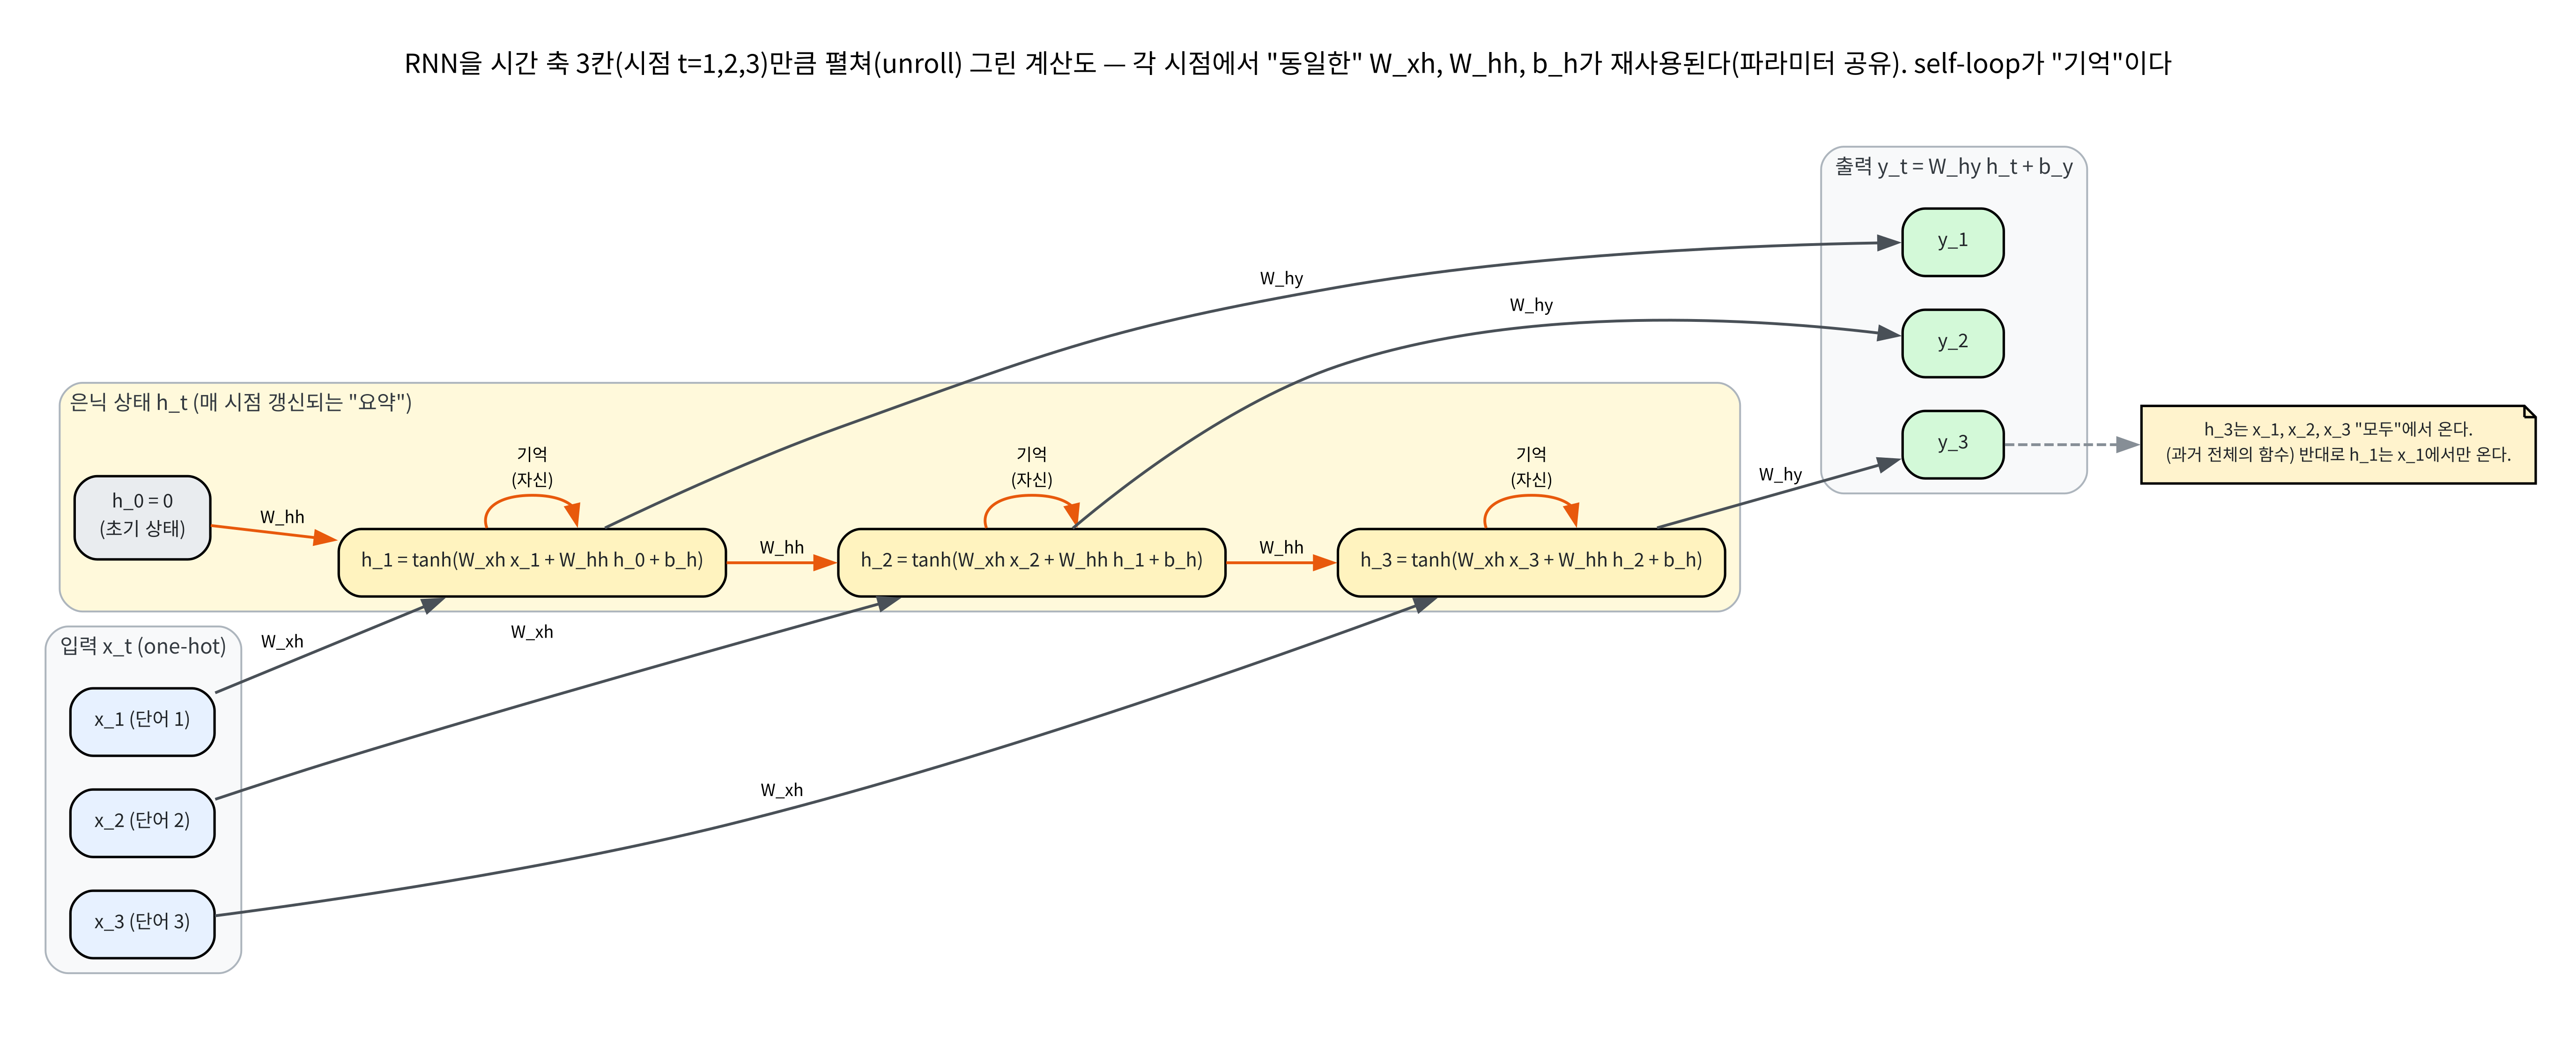
\includegraphics[width=\linewidth]{ch11_1_rnn_unroll.png}
      \vskip0.3em
      {\footnotesize $h_t$의 self-loop = ``기억''의 시각화.
      $h_0 = 0$에서 시작.}
    \end{column}
    \begin{column}{0.5\textwidth}
      시퀀스 전체를 한눈에 보는 가장 좋은 방법: \textbf{시간을
      펼쳐서(unroll) 그리는 것}.
      \begin{itemize}
        \item \textbf{같은 네트워크}가 시점마다 반복되어 있는 것이지,
          각 시점에 \textbf{별개의 층}이 있는 것이 아님
        \item 출력 $y_t$는 $x_1, x_2, \ldots, x_t$ \textbf{전부}에서
          온다 --- $y_3$는 $h_3$를 통해 $x_1, x_2$의 영향도 받음
        \item 반대로 $y_1$은 $x_1$에서만 온다
      \end{itemize}
      \vskip0.4em
      \kq{``과거만 보고 미래는 못 본다''는 시간의 비가역성이
      이 도식 안에 정확히 들어 있다.}
    \end{column}
  \end{columns}
\end{frame}

\begin{frame}{파라미터 수: 시퀀스 길이와 무관}
  문자 단위 언어모델(어휘 $V=26$ — a$\sim$z, 은닉 크기 $H=8$)의
  파라미터를 세어보자:
  \vskip0.5em
  \small
  \begin{tabular}{@{}lll@{}}
    \toprule
    매개변수 & 크기 & 개수 \\
    \midrule
    $W_{xh}$ (입력 $\to$ 은닉) & $H \times V$ & 8 $\times$ 26 = 208 \\
    $W_{hh}$ (은닉 $\to$ 은닉) & $H \times H$ & 8 $\times$ 8 = 64 \\
    $W_{hy}$ (은닉 $\to$ 출력) & $V \times H$ & 26 $\times$ 8 = 208 \\
    $b_h$ & $H$ & 8 \\
    $b_y$ & $V$ & 26 \\
    \midrule
    \textbf{합계} & & \textbf{514} \\
    \bottomrule
  \end{tabular}
  \vskip0.6em
  \begin{itemize}
    \item 10글자든 1000글자든 \textbf{514개} --- 파라미터가 시퀀스
      길이에 비례하지 않는 것이 파라미터 공유의 직접적 혜택
    \item 비교: 같은 문자열을 MLP에 넣으려면 ``직전 5글자'' 윈도우를
      펼쳐 $5 \times 26 = 130$차원 입력으로 --- 더 긴 맥락은 윈도우
      확대로 입력 차원이 선형 증가
    \item 첫 은닉층만 8개 뉴런이어도 $130 \times 8 + 8 = 1048$개
      --- \textbf{파라미터 수만 이미 RNN 전체(514)의 두 배}
  \end{itemize}
\end{frame}

\begin{frame}[fragile]{코드: 한 걸음($rnn\_step$)과 전체($rnn\_forward$)}
\begin{lstlisting}
def rnn_step(x_t, h_prev, Wxh, Whh, b_h):
    z = [sum(Wxh[i][j]*x_t[j] for j in range(len(x_t))) +
         sum(Whh[i][j]*h_prev[j] for j in range(len(h_prev))) + b_h[i]
         for i in range(len(h_prev))]
    return [tanh(v) for v in z]

def rnn_forward(inputs, h0, Wxh, Whh, b_h):
    h = h0
    hidden_states = []
    for x_t in inputs:
        h = rnn_step(x_t, h, Wxh, Whh, b_h)
        hidden_states.append(h)
    return hidden_states
\end{lstlisting}
  \begin{itemize}
    \item 한 줄로 요약: \textbf{``같은 $rnn\_step$을 $T$번 순서대로
      반복하는 것''}
    \item 이 \textbf{순차성}($t=1$이 끝나야 $t=2$를 시작)이 RNN의
      장점(파라미터 효율)이자 동시에 단점(\textbf{병렬화 불가} ---
      11.3절)
  \end{itemize}
\end{frame}

\begin{frame}{``무엇을'' 담느냐: 누적합 예제}
  ``과거의 요약''은 추상적이다 --- 아주 단순한 \kb{누적합(running
  sum)}을 RNN 구조가 어떻게 수행하는지 스칼라 예제로 직접 추적.
  (11.2절에서 같은 구조를 \textbf{학습}시키는 모델이 등장한다.)
  \vskip0.4em
  \begin{itemize}
    \item 스칼라 RNN, $w_{xh}=0.1$, $w_{hh}=0.9$, $b_h=0$,
      입력 $[2, 3, 1, 4]$
    \item pre-activation $z_t$(\,\tanh 전\,)를 따라가면:
  \end{itemize}
  \[ z_1 = 0.200, \qquad z_2 = 0.480, \qquad z_3 = 0.532,
     \qquad z_4 = 0.879 \]
\end{frame}

\begin{frame}{기억의 감쇠 구조}
  $z_t = 0.1\, x_t + 0.9\, z_{t-1}$에 $z_{t-1}$을 재귀적으로 대입하면:
  \vskip0.4em
  \[ z_t = 0.1\, x_t + 0.1 \cdot 0.9\, x_{t-1}
           + 0.1 \cdot 0.9^{\,2}\, x_{t-2} + \cdots \]
  \vskip0.4em
  \begin{itemize}
    \item \kq{주의: $\tanh$가 없어야 성립하는 \textbf{근사}.} 실제로는
      $h_t = \tanh(z_t)$라 재귀는 비선형 --- $z$가 작은
      ($\tanh z \approx z$) 구간에서만 좋은 근사
    \item 그래도 \textbf{감쇠의 구조}는 정확히 보인다: $z_t$는 과거
      입력들의 \textbf{기하급수적으로 감쇠된 가중합}
    \item $0.9^{\,k}$ = $k$칸 전 입력의 ``\textbf{기억 세기}''
    \item $k=10$: $0.9^{10} \approx 0.35$ (10단어 전 정보의 35%
      잔존), $k=20$: $\approx 0.12$
    \item $w_{hh}$를 0.5로 바꾸면 $0.5^{10} \approx 0.001$ ---
      \textbf{거의 잊는다}
  \end{itemize}
  \vskip0.4em
  \kq{``기억의 길이''는 $w_{hh}$ 하나의 값으로 조절된다 ---
  11.3절 ``그래디언트도 같은 $W_{hh}$의 곱으로 소실된다''의 열쇠.}
\end{frame}

\begin{frame}{$\tanh$를 거친 은닉 상태: 포화}
  실제로 $\tanh$를 거치면 $h_t = \tanh(z_t) =
  [0.197,\; 0.444,\; 0.462,\; 0.673]$.
  \begin{itemize}
    \item 이 $h_t$를 누적합 추정치로 ($\hat{s}_t = 10 \cdot h_t$):
      누적합 $[2, 5, 6, 10]$의 추정 $\to$
      $[1.97,\; 4.44,\; 4.62,\; 6.73]$
    \item 초기에는 거의 정확하고, 입력이 클수록 $\tanh$의 \textbf{포화}
      로 점점 아래로 벗어남 --- 두 원인:
    \begin{enumerate}
      \item $\tanh$의 ``요약 벡터는 $[-1, 1]$ 안에 갇힌다''는 한계
      \item 큰 숫자의 누적합을 \textbf{저차원 벡터 하나}에 담으려
        할 때의 왜곡
    \end{enumerate}
    \item 실전 RNN은 \textbf{여러 차원} 은닉 상태(11.2절 $H=8$) +
      11.3절의 \textbf{게이트} 구조로 이 문제를 다룬다
    \item \kq{주의: 11.2절의 ``abcabc…'' 모델은 이 누적합을 스스로
      학습한 것이 아니라 \textbf{단 3글자 주기라는 더 쉬운 요령}을
      배운다 --- 같은 구조라도 데이터에 따라 ``기억''의 내용이
      바뀐다.}
  \end{itemize}
\end{frame}

\begin{frame}{손으로 한 번: 스칼라 RNN 세 스텝}
  은닉 상태가 \textbf{스칼라(숫자 하나)}인 가장 단순한 RNN.
  $w_{xh}=0.5$, $w_{hh}=0.8$, $b_h=0$, 입력이 매 시점 $x_t=1.0$으로
  고정, $h_0=0$에서 시작:
  \vskip0.5em
  \[ h_1 = \tanh(0.5 \times 1.0 + 0.8 \times 0)
          = \tanh(0.5) \approx 0.462 \]
  \[ h_2 = \tanh(0.5 \times 1.0 + 0.8 \times 0.462)
          = \tanh(0.870) \approx 0.701 \]
  \[ h_3 = \tanh(0.5 \times 1.0 + 0.8 \times 0.701)
          = \tanh(1.061) \approx 0.786 \]
  \vskip0.5em
  \begin{itemize}
    \item 같은 입력($x_t = 1.0$)이 반복되는데도 $h_t$가 매 시점 다른
      값으로 갱신 (0.462 $\to$ 0.701 $\to$ 0.786)
    \item 이유: ``이전 은닉 상태''가 매번 입력에 \textbf{새로
      더해지기} 때문
    \item 점점 커지다가 어떤 값 근처로 \textbf{수렴}해간다 ---
      $\tanh$가 큰 입력에서 \textbf{포화(saturate)}되어 1에
      가까워지기 때문
  \end{itemize}
  \vskip0.3em
  {\footnotesize 이 ``포화'' 현상이 11.3절의 그래디언트 소실과 정확히
  같은 뿌리(미분이 0에 가까워짐)를 공유한다.}
\end{frame}

\begin{frame}{고정점과 그 ``속도''}
  위 계산을 10단계까지 이어가면 ($w_{xh}=0.5$, $w_{hh}=0.8$):
  \vskip0.4em
  \small
  \begin{tabular}{@{}l|cccccccc@{}}
    \toprule
    $t$ & 1 & 2 & 3 & 4 & 5 & 6 & 8 & 10 \\
    \midrule
    $z_t = 0.5 + 0.8\,h_{t-1}$ & 0.500 & 0.870 & 1.061 & 1.129 & 1.149 & 1.154 & 1.156 & 1.156 \\
    $h_t = \tanh(z_t)$ & 0.462 & 0.701 & 0.786 & 0.811 & 0.817 & 0.819 & 0.820 & 0.820 \\
    \bottomrule
  \end{tabular}
  \vskip0.5em
  \begin{itemize}
    \item $h_t$는 \kb{고정점(fixed point)}
      $h^\ast = \tanh(0.5 + 0.8\, h^\ast)$으로 수렴 --- 해는
      $h^\ast \approx 0.8196$, $t=10$에서 차이 $< 10^{-3}$
    \item ``같은 입력이 계속 오면 은닉 상태가 결국 한 곳에
      정지한다'' --- RNN의 \textbf{동적(dynamics)}을 이해하는
      출발점
    \item 수렴 \textbf{속도}는 고정점 근처의 ``\textbf{증폭 인자}''로
      결정: $\frac{d h_t}{d h_{t-1}} = 0.8 \cdot \tanh'(z_t)$
    \item $h^\ast \approx 0.82$에서 $\tanh'(z^\ast) = 1 - (h^\ast)^2
      \approx 0.325$ $\Rightarrow$ 증폭 인자 $0.8 \times 0.325
      \approx 0.26$ --- 각 단계마다 차이가 약 4분의 1로 줄어듦
      (표에서 $h_5$ 이후가 거의 움직이지 않는 이유)
  \end{itemize}
\end{frame}

\begin{frame}{핵심: 이 ``증폭 인자''가 11.3절의 그래디언트 소실과
\textbf{정확히 같은 수식}}
  \begin{itemize}
    \item \textbf{순전파}: $h_{t-1}$의 작은 변화가 $h_t$에 얼마나
      전달되는지 재는 $\tanh'(z_t) \cdot w_{hh}$의 곱
    \item \textbf{역전파}: 손실의 그래디언트가 시점을 거슬러 올라갈
      때 곱해지는 인자 $\tanh'(z_t) \cdot W_{hh}$ (11.2절)
    \item $\to$ \textbf{구조적으로 동일}: 순전파의 ``기억이 빠르게
      잊히는 속도''와 역전파의 ``그래디언트가 빠르게 사라지는
      속도''는 \textbf{같은 연쇄법칙 곱의 두 얼굴}
    \item 11.3절이 다룰 그래디언트 소실을 \textbf{11.1절의 순전파에서
      미리 체감}하고 있는 셈 --- $\tanh$의 포화는 수렴을
      \textbf{부추기는} 동시에 그래디언트 소실을 \textbf{조성하는}
      동일한 원인
  \end{itemize}
\end{frame}

\begin{frame}{$w_{hh}$를 0.9로 키우면? --- 그리고 발산}
  \begin{columns}[T]
    \begin{column}{0.55\textwidth}
      \begin{itemize}
        \item 고정점은 $h^\ast \approx 0.853$으로 조금 높아짐
        \item 증폭 인자 $0.9 \times (1 - 0.853^2) \approx 0.245$ ---
          0.8 경우(0.263)보다 오히려 약간 \textbf{작아짐}
        \item 둘 다 6단계 만에 고정점의 $10^{-3}$ 이내로 \textbf{정착}
        \item ``\textbf{발산}''은 여전히 하지 않는다: 증폭 인자가 1보다
          작기 때문
        \item 스칼라 RNN은 $\tanh$의 범위 $[-1, 1]$에 갇혀 있어
          발산 자체가 \textbf{불가능}
      \end{itemize}
      \vskip0.5em
      \kq{단, 은닉 크기가 큰($H > 1$) RNN에서는 $W_{hh}$의
      \textbf{고유값이 1보다 크면} $h_t$가 실제로 발산하거나
      진동할 수 있다 --- 11.2절 ``자주 하는 실수''의 그래디언트
      폭발과 같은 뿌리 (Pascanu et al., 2013).}
    \end{column}
    \begin{column}{0.45\textwidth}
      \centering
      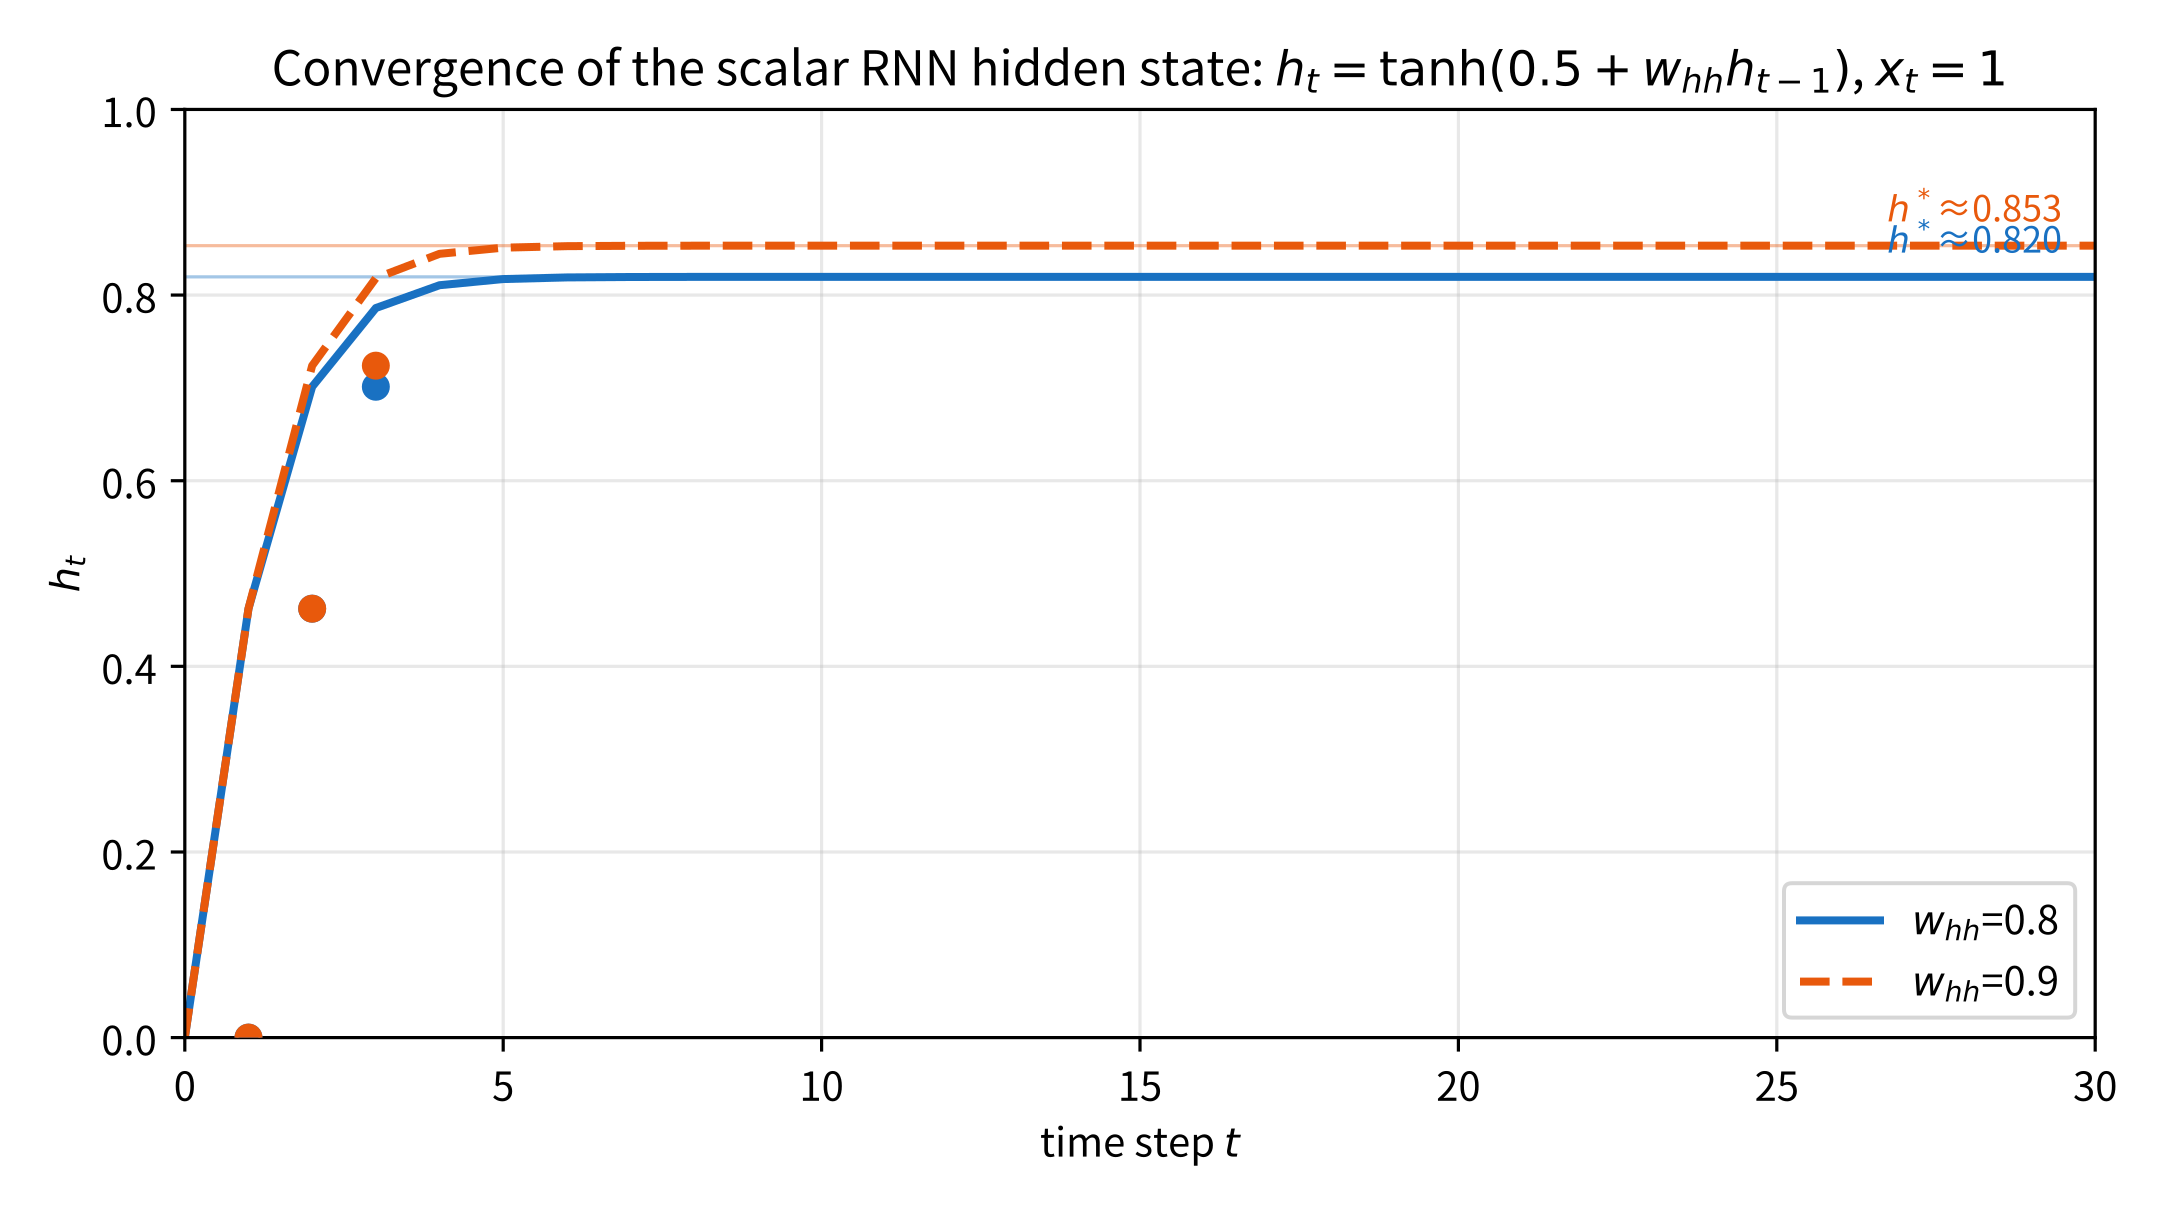
\includegraphics[width=\linewidth]{ch11_1_scalar_convergence.png}
      \vskip0.3em
      {\footnotesize $w_{hh}=0.8$: 0.820으로, $w_{hh}=0.9$: 0.853으로
      수렴 --- 약 6단계 만에 정착.}
    \end{column}
  \end{columns}
\end{frame}

\begin{frame}{자주 하는 실수 1: ``$h_t$는 $x_t$만 의존한다''}
  RNN을 처음 접할 때 가장 흔한 오해: 순전파 수식에서
  $W_{hh}\, h_{t-1}$ 항을 ``보조적인 정규화 항''쯤으로 여기는 것.
  \vskip0.6em
  \begin{itemize}
    \item $h_t$는 \textbf{과거 전체 $(x_1, \ldots, x_t)$의 함수}이며,
      $x_t$ 하나만 의존하지 않는다
    \item ``은닉 상태가 과거를 기억한다''는 이 절의 모든 주장이
      \textbf{이 한 항}에 달려 있다
    \item $W_{hh} = 0$으로 두면:
      $h_t = \tanh(W_{xh}\, x_t + b_h)$로
      \textbf{``시점을 독립적으로 처리하는 MLP''로 퇴화}
    \item 결과: 10단어 문장의 10번째 단어를 예측할 때 \textbf{앞의
      9단어를 완전히 잊는} 모델
  \end{itemize}
  \vskip0.6em
  \kq{$W_{hh}\, h_{t-1}$을 빼면 RNN은 RNN이 아니다.}
\end{frame}

\begin{frame}{자주 하는 실수 2: ``시점마다 가중치가 달라진다''}
  전개도에서 각 시점에 하나의 ``박스''가 그려져 있어서, ``시점 1에는
  $W^{(1)}_{xh}$, 시점 2에는 $W^{(2)}_{xh}$…'' 같은 \textbf{별개의
  가중치}가 있는 것으로 오해하기 쉽다.
  \vskip0.5em
  \begin{itemize}
    \item 아니다 --- \textbf{세 행렬 $W_{xh}, W_{hh}, W_{hy}$가 시점
      전체에서 공유}된다 (파라미터 공유)
    \item 이 공유 덕분에:
    \begin{enumerate}
      \item 시퀀스 길이에 관계없이 \textbf{파라미터 수가 일정}
      \item ``5번째 단어를 처리하는 능력''이 ``150번째 단어를 처리하는
        능력''에도 \textbf{자동으로 전이}
    \end{enumerate}
    \item 이 공유가 없다면: RNN은 ``시퀀스 길이 = 층 수''로 고정된,
      학습할 파라미터가 시퀀스 길이에 \textbf{비례하는 단순 MLP
      스택}과 다를 바가 없다
  \end{itemize}
\end{frame}

\begin{frame}[fragile]{실습: 숫자 하나씩 코드로}
  3단계 손계산 · 고정점 · 누적합 예제를 하나의 코드로:
\begin{lstlisting}
import math

def rnn_step(x, h, wxh, whh, b=0.0):
    return math.tanh(wxh * x + whh * h + b)

# 3단계 손계산 (w_xh=0.5, w_hh=0.8, x=1, h0=0)
h = 0.0
for _ in range(3):
    h = rnn_step(1.0, h, 0.5, 0.8)
    print(f"h = {h:.4f}")       # 0.4621 / 0.7012 / 0.7860

# 고정점 반복 대입: h = tanh(0.5 + 0.8h)
h = 0.0
for _ in range(100):
    h = rnn_step(1.0, h, 0.5, 0.8)
print(f"고정점 h* ~ {h:.4f}")   # 0.8196

# 누적합 예제 (w_xh=0.1, w_hh=0.9), 입력 [2,3,1,4]
h = 0.0
for x in [2.0, 3.0, 1.0, 4.0]:
    h = rnn_step(x, h, 0.1, 0.9)
    print(f"h = {h:.4f}")       # 0.1974 / 0.4444 / 0.4621 / 0.6728
\end{lstlisting}
  {\footnotesize 완전 버전(수렴 곡선 + unroll 다이어그램 포함)은
  실습 노트북에서 실행.}
\end{frame}

\begin{frame}{핵심 공식 한눈에}
  \small
  \begin{tabular}{@{}p{2.6cm}p{7.2cm}p{4.6cm}@{}}
    \toprule
    항목 & 공식 & 무엇을 말하나 \\
    \midrule
    순전파 (재귀) & $h_t = \tanh(W_{xh} x_t + W_{hh} h_{t-1} + b_h)$ &
      시점마다 은닉 상태 갱신 \\
    출력 & $y_t = W_{hy} h_t + b_y$ & 시점별 예측 (선형, 활성함수 없음) \\
    파라미터 & $(HV + 1) + H^2 + (VH + 1)$ & \textbf{시퀀스 길이 $T$와
      무관} \\
    기억의 감쇠 & $z_t \approx \sum_{k} w_{hh}^{\,k-1} \cdot w_{xh}\,
      x_{t-k+1}$ & $w_{hh}$가 ``기억의 길이''를 결정 \\
    \bottomrule
  \end{tabular}
  \vskip1em
  \begin{block}{한 줄}
    RNN = \textbf{같은 세 행렬을 $T$번 순서대로 돌리며}, 이전 요약을
    $\tanh$로 압축해 갱신하는 구조.
  \end{block}
\end{frame}

\begin{frame}{FAQ: 은닉 상태 크기와 인코더-디코더}
  \begin{block}{Q. 은닉 상태의 크기는 어떻게 정하나요?}
    ``지금까지의 맥락을 얼마나 \textbf{풍부하게 요약}할 수 있는가''를
    결정하는 하이퍼파라미터 --- Ch.\,9의 은닉층 뉴런 수와 같은
    종류의 선택.
    \begin{itemize}
      \item 너무 작으면 \textbf{긴 문맥을 다 담지 못}하고
      \item 너무 크면 파라미터 증가 $\to$ \textbf{과적합 · 계산비용}
        문제
    \end{itemize}
  \end{block}
  \vskip0.6em
  \begin{block}{Q. 입력과 출력이 다른 경우(번역)는?}
    ``입력을 끝까지 읽고 \textbf{마지막 은닉 상태 하나}로부터 새
    시퀀스를 순차 생성''하는 \kb{인코더-디코더(encoder-decoder)}
    구조를 쓰면 가능 --- 단, 긴 입력을 하나의 벡터로 압축하면
    \textbf{정보 손실}이 생김.
    \kq{Ch.\,12의 Attention이 정확히 이 한계를 보완하기 위해
    출발했다} (Bahdanau et al., 2014).
  \end{block}
\end{frame}

\begin{frame}{FAQ: 문장 전체를 펼쳐 MLP에 넣으면 안 되는가}
  세 가지 이유다:
  \begin{enumerate}
    \item \kb{파라미터} --- 문장 길이 $T$ $\times$ 임베딩 차원 $d$개
      입력을 100개 뉴런의 은닉층에 연결하면 $100\,T\,d$개 가중치 ---
      $T$에 \textbf{비례해 팽창}. RNN은 $T$와 무관하게
      $HV + H^2 + VH$개만
    \item \kb{길이 가변성} --- 실제 문장은 길이 불균일: 5단어와
      200단어 입력을 하나의 MLP로 처리하려면 \textbf{패딩}이나
      \textbf{분리된 모델}이 필요. RNN은 같은 가중치로 어떤
      길이든 처리
    \item \kb{위치 인코딩 불필요} --- MLP에 ``100번째 단어''를
      넣으려면 ``이건 100번째 위치의 단어''라는 정보(위치 인코딩,
      Ch.\,12)를 \textbf{별도로} 줘야. RNN은 \textbf{순차적 처리
      자체}가 위치 정보를 자동 반영
  \end{enumerate}
  \vskip0.5em
  {\footnotesize 그럼에도 ``RNN은 순차적이라 느리다''는 이유로
  Transformer가 주류가 된 이유도 11.3절에서 본다.}
\end{frame}

\begin{frame}{FAQ: 왜 $\tanh$인가, $h_0$는 항상 0인가}
  \begin{block}{Q. 왜 $\tanh$인가? 시그모이드($0\sim1$)도 되는데}
    \begin{enumerate}
      \item \kb{중심화}: $\tanh$ 출력 범위 $[-1, 1]$은 0 중심 대칭.
        시그모이드 $[0, 1]$은 항상 양수 $\to$ 여러 성분이 ``동일
        방향''으로 움직이는 경향, 학습이 느려짐 (9.2절의 시그모이드
        ``비대칭 골짜기'')
      \item \kb{미분의 크기}: $\tanh'$ 최댓값 1 = 시그모이드 미분
        최댓값 0.25의 \textbf{4배} --- 같은 깊이에서 그래디언트가
        4배 강하게 전달
    \end{enumerate}
    반대로 \textbf{출력층} $y_t = W_{hy} h_t + b_y$는 활성함수 없이
    \textbf{선형}: ``다음 문자의 확률 분포(softmax)''나 ``실수값(회귀)''
    으로 해석되어야 하므로 $[-1, 1]$로 자르는 $\tanh$가 오히려
    방해 --- 은닉층과 출력층은 \textbf{역할}이 다르다.
  \end{block}
  \vskip0.5em
  \begin{block}{Q. $h_0$는 항상 0이어야 하나요?}
    꼭 아니다 --- ``시퀀스를 읽기 \textbf{전}에 알고 있는 것''을 담을
    수 있는 초기 조건: (a) 0으로 고정 (가장 흔함), (b) \textbf{학습
    가능} 파라미터 벡터, (c) \textbf{이전 시퀀스의 최종 은닉
    상태}를 이어받아 이어지는 시퀀스 처리 (음성인식: 전 문장의
    마지막 상태를 다음 문장의 초기 상태로).
  \end{block}
\end{frame}

% ============================================================
\section{11.2 BPTT와 numpy RNN 언어모델 실습}

\begin{frame}{BPTT: 시간을 펼쳐서 역전파하기}
  ``요약을 계속 갱신한다''는 구조를 \textbf{배우게} 만들려면
  순전파만으로는 부족하다.
  \begin{itemize}
    \item 손실을 줄이려면 각 가중치에 대한 \textbf{그래디언트}를
      구해야
    \item $h_t$가 $h_{t-1}$에, $h_{t-1}$이 $h_{t-2}$에 의존하는
      \textbf{사슬}을 이룸
    $\Rightarrow$ Ch.\,9의 ``출력층 $\to$ 입력층'' 역전파를
    \textbf{시간 축을 따라 펼쳐} 적용
  \end{itemize}
  \vskip0.5em
  \begin{block}{BPTT(Backpropagation Through Time)}
    시퀀스 길이 $T$만큼 신경망을 \textbf{펼쳐서(unroll)} 각 시점을
    독립된 층처럼 취급한 뒤 Ch.\,9의 역전파를 \textbf{그대로}
    적용.
  \end{block}
  \vskip0.5em
  \[ \frac{\partial h_T}{\partial h_1} = \prod_{t=2}^{T}
     \frac{\partial h_t}{\partial h_{t-1}}
     = \prod_{t=2}^{T} \operatorname{diag}\big(\tanh'(z_t)\big)\; W_{hh} \]
  \vskip0.3em
  {\footnotesize $z_t = W_{xh}x_t + W_{hh}h_{t-1} + b_h$,
  $\tanh'(z_t) = 1 - h_t^2$.}
\end{frame}

\begin{frame}{곱적: 소실·폭발의 씨앗}
  이 식이 말해주는 것: \textbf{먼 시점과 가까운 시점 사이를
  건너는 그래디언트는 $W_{hh}$를 $T-1$번 곱하는 곱적}이 된다.
  \vskip0.6em
  \begin{columns}[T]
    \begin{column}{0.5\textwidth}
      \begin{block}{$W_{hh}$ 고유값 $< 1$}
        곱이 \textbf{지수적으로 0}으로 --- ``그래디언트 \textbf{소실}''
      \end{block}
      \vskip0.5em
      \begin{block}{$W_{hh}$ 고유값 $> 1$}
        곱이 \textbf{지수적으로 $\infty$}로 발산 --- ``그래디언트
        \textbf{폭발}''
      \end{block}
    \end{column}
    \begin{column}{0.5\textwidth}
      11.3절에서 ``그래디언트 소실·폭발''이라는 이름으로 다시 만나는
      바로 그 문제 (Pascanu et al., 2013).
      \vskip0.5em
      \kq{이번 절: 그 \textbf{양}보다 먼저, 이 곱적 구조를
      \textbf{정확히} 따라가며 각 파라미터의 그래디언트가 어떻게
      \textbf{누적}되는지 유도한다.}
    \end{column}
  \end{columns}
\end{frame}

\begin{frame}{펼쳐진 계산 그래프: 시점이 곧 ``층''}
  \begin{columns}[T]
    \begin{column}{0.48\textwidth}
      \centering
      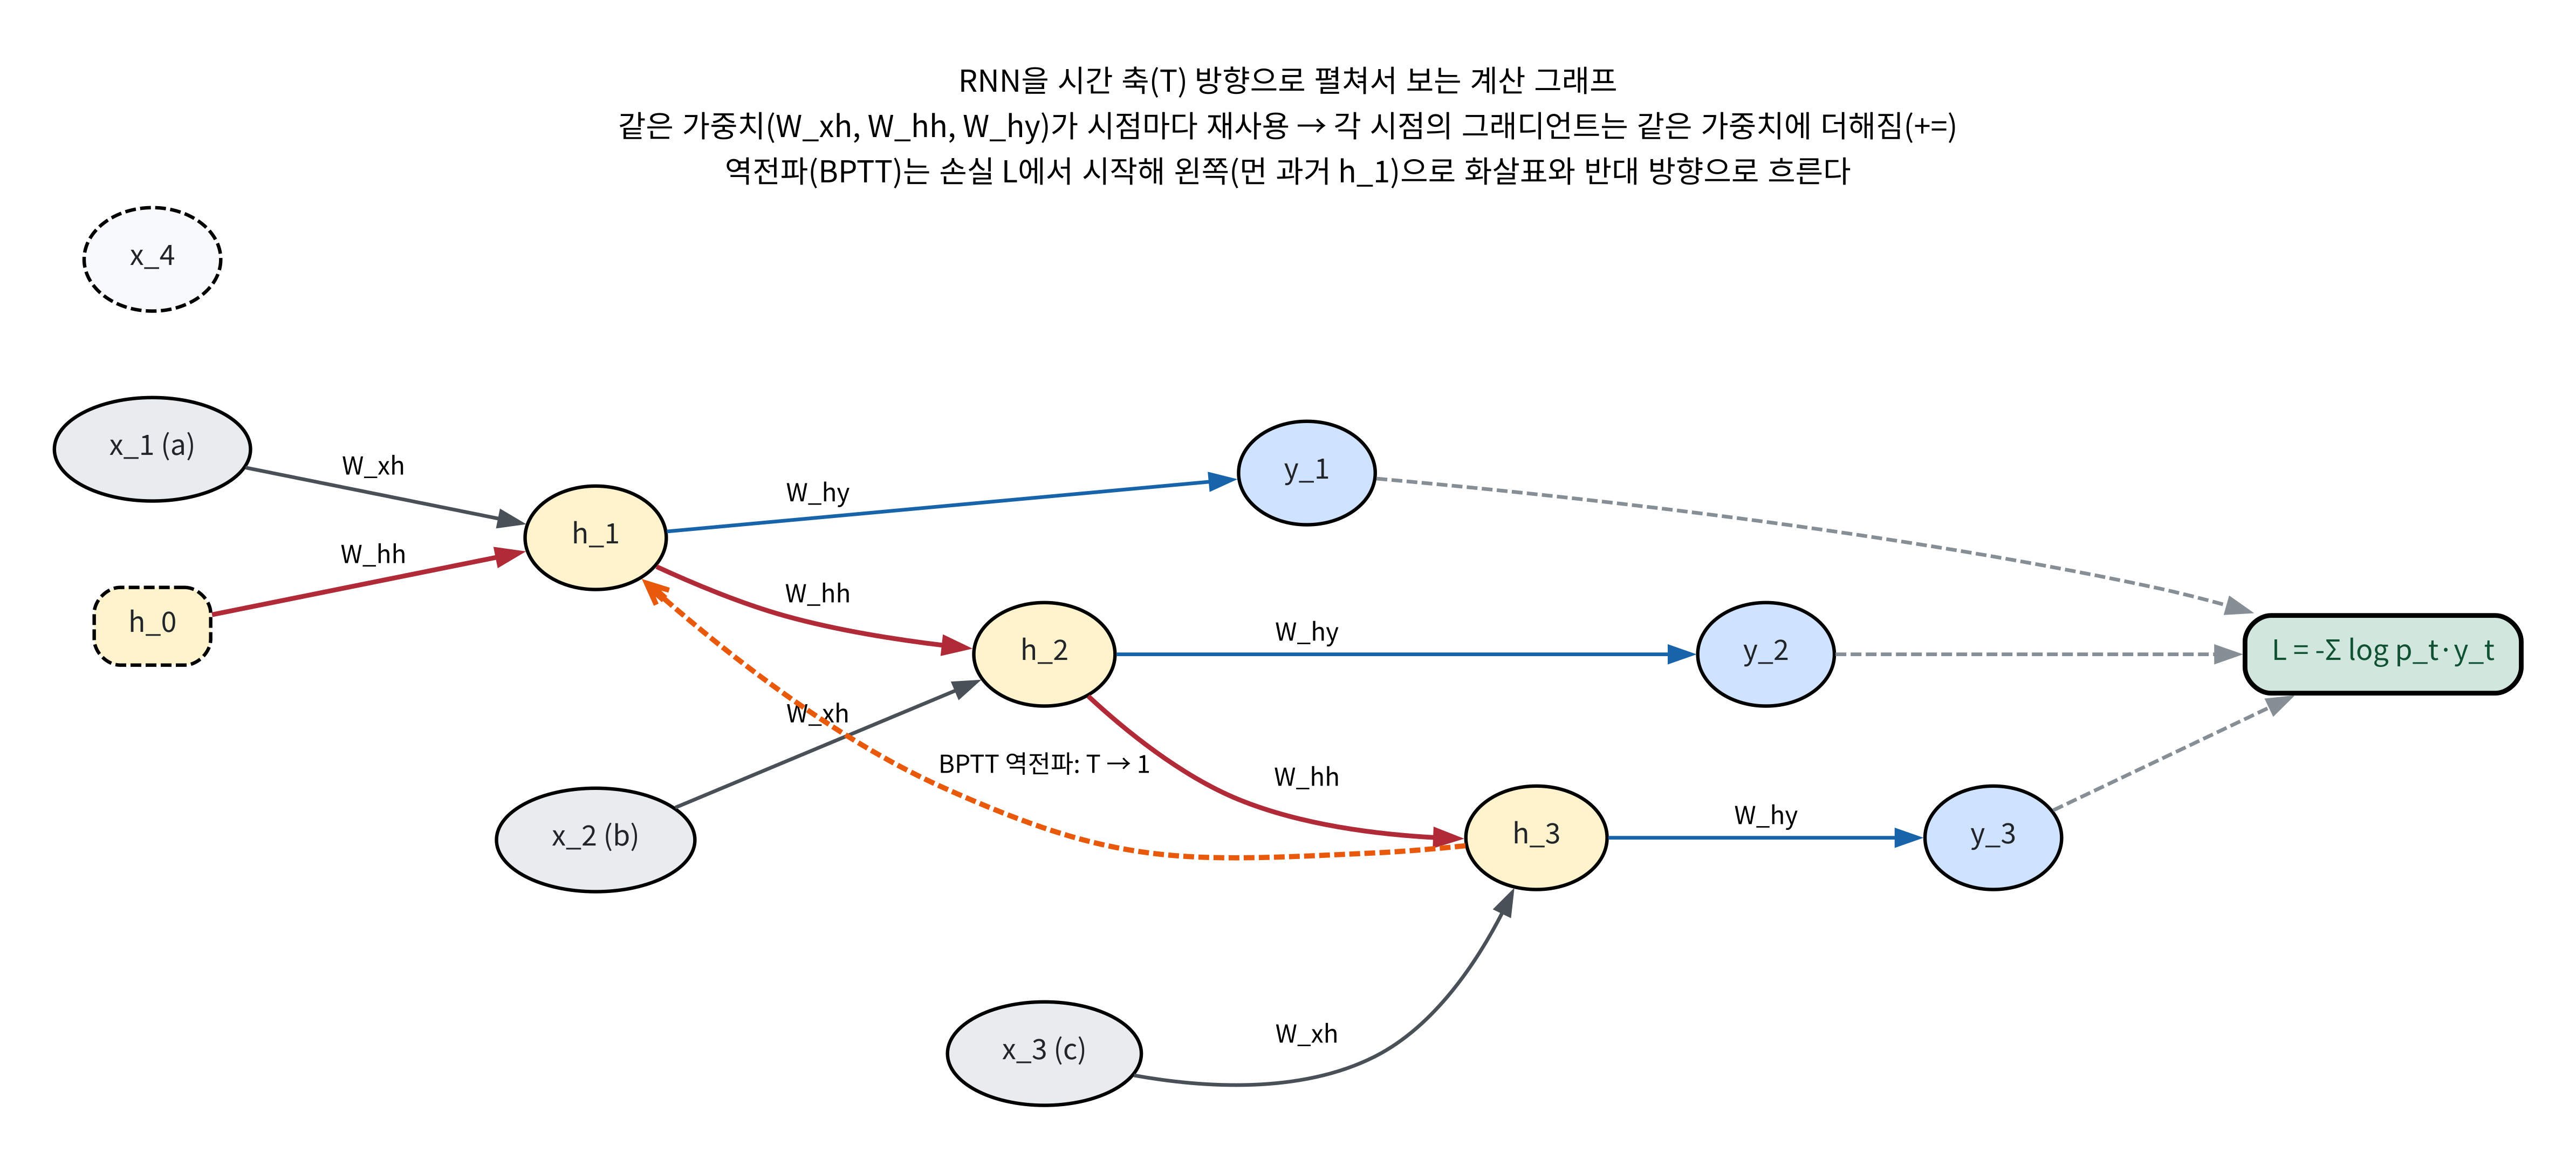
\includegraphics[width=\linewidth]{ch11_2_bptt_unroll.png}
      \vskip0.3em
      {\footnotesize 역전파는 오른쪽(손실)에서 왼쪽(과거)으로.}
    \end{column}
    \begin{column}{0.52\textwidth}
      중요한 것 세 가지:
      \begin{enumerate}
        \item \kb{수직 화살표($W_{hh}$)}: 자기-루프
          ($h_{t-1} \to h_t$). 역전파에서는 \textbf{위에서
          아래로} --- $h_t$에서 $h_{t-1}$으로 거슬러 올라감
        \item \kb{각 시점의 출력 화살표($W_{hy}$)}: $h_t \to y_t$.
          손실이 \textbf{모든 시점}의 $y_t$에서 나므로 역전파는
          이 화살표들에서 시작
        \item \kb{같은 색 박스가 모든 시점에서 반복}: 시점 1과
          시점 2의 $W_{xh}, W_{hh}, W_{hy}$는 \textbf{동일한}
          가중치 (파라미터 공유) $\Rightarrow$ 각 시점의 그래디언트는
          \textbf{같은 가중치의 그래디언트에 더해짐}
      \end{enumerate}
      \vskip0.3em
      \kq{이 ``누적''이 BPTT에서 가장 실수하기 쉬운 지점.}
    \end{column}
  \end{columns}
\end{frame}

\begin{frame}{BPTT 유도: 시점마다 ``(A) + (B)''}
  손실을 \textbf{모든 시점}의 크로스엔트로피 합으로 놓는다:
  \vskip0.4em
  \[ L = -\sum_{t=1}^{T} \sum_{k} y_{t,k}^{\,\text{true}} \log p_{t,k} \]
  {\footnotesize $p_t = \operatorname{softmax}(W_{hy} h_t + b_y)$ =
  시점 $t$의 다음-문자 분포, $y_t^{\,\text{true}}$ = 원-핫 정답.}
  \vskip0.4em
  역전파는 \textbf{마지막 시점 $T$에서 첫 시점 1로} 순차적으로
  내려간다. 핵심 --- 각 시점 $t$의 은닉 상태 그래디언트는
  \textbf{두 부분의 합}:
  \vskip0.4em
  \[ \underbrace{W_{hy}^{\top}\big(p_t - y_t^{\,\text{true}}\big)}_{(A)\;\text{본 시점의 출력 오차}}
     \;+\; \underbrace{W_{hh}^{\top}\Big[\frac{\partial L}{\partial h_{t+1}}
     \odot (1 - h_{t+1}^{\,2})\Big]}_{(B)\;\text{시점 } t{+1} \text{에서 흘러온 그래디언트}} \]
\end{frame}

\begin{frame}{Ch.\,9의 2층 역전파와 같은 형태}
  \begin{itemize}
    \item ``다음 시점에서 온 그래디언트 $+$ 그 시점 자체의 출력
      오차''를 합친다는 점에서, 각 시점의 역전파는 \textbf{Ch.\,9.1의
      2층 신경망 역전파와 형태가 같다}
    \item 다만 ``은닉층에서 입력층으로'' 대신 \textbf{``시점 $t$에서
      시점 $t-1$으로''} 거슬러 올라간다는 점이 다를 뿐
    \item 재귀 구조: (B) 항이 \textbf{다음 시점의 $(A)+(B)$}를
      다시 포함 --- 사슬이 이렇게 한 시점씩 이어진다
  \end{itemize}
  \vskip0.6em
  \begin{block}{핵심 문장}
    본 시점 오차 $(A)$에, \textbf{더 새로운 시점}에서 흘러온
    그래디언트 $(B)$를 \textbf{더하고}, $W_{hh}$가 공유되므로 그
    기여는 \textbf{같은 텐서에 누적}($+=$)된다.
  \end{block}
\end{frame}

\begin{frame}[fragile]{BPTT 코드: 핵심 루프}
\begin{lstlisting}
# 역전파: t = T-1, T-2, ..., 0 순으로 (0-indexed)
dh_next = np.zeros(H)                 # dL/dh_{t+1} (첫 루프: 0)
dWxh = dWhh = dWhy = 0; dbh = dby = 0
for t in reversed(range(T)):
    p = softmax(Why @ hs[t] + by)
    dp = p.copy(); dp[targets[t]] -= 1  # p_t - onehot
    dWhy += np.outer(dp, hs[t]); dby += dp        # (A)
    dh = Why.T @ dp + dh_next               # (A)+(B)의 합
    dz = dh * (1 - hs[t]**2)                # * tanh'(z_t)
    dh_next = Whh.T @ dz                    # -> 이전 시점 B로 전달
    dWhh += np.outer(dz, hps[t]); dbh += dz
    dWxh += np.outer(dz, one_hot(inputs[t]))
\end{lstlisting}
  \begin{itemize}
    \item \kb{첫째} \verb|dh = Why.T @ dp + dh_next|: 본 시점 오차에
      \textbf{더 새로운 시점}에서 흘러온 그래디언트를 더하는 $(A)+(B)$
    \item \kb{둘째} \verb|dWhh += ...| 는 \verb|=|가 아니라 \verb|+=|
      --- $W_{hh}$가 \textbf{모든 시점에서 공유}되므로 각 시점의
      기여를 \textbf{같은 텐서에 계속 더해야} 함
  \end{itemize}
\end{frame}

\begin{frame}{왜 \texttt{p - onehot}인가: softmax + CE}
  크로스엔트로피($-\log p_k$, $k$가 정답)를 softmax 출력 $p_j$로
  미분하면 \textbf{경악할 정도로 깔끔한} 결과:
  \vskip0.4em
  \[ \frac{\partial L}{\partial z_j} = p_j - \mathbb{1}[j = k] \]
  \vskip0.4em
  ``softmax의 출력에서 \textbf{정답 클래스 자리에만 1을 빼고}
  나머지는 그대로''.
  \begin{itemize}
    \item Ch.\,9.1의 로지스틱 회귀 + 크로스엔트로피 그래디언트
      ``(예측 $-$ 정답)''와 \textbf{정확히 같은 패턴}의 다항분류
      버전
    \item 왜 단순해지는가: 연쇄법칙으로 펼치면
      $\sum_k (-y_k/p_k)\, p_k(\delta_{kj} - p_j)$
      $= -\underbrace{\sum_k y_k \delta_{kj}}_{y_j}
       + p_j \underbrace{\sum_k y_k}_{1} = p_j - y_j$
    \item softmax의 $p_k$가 크로스엔트로피의 $1/p_k$와
      \textbf{상쇄}되기 때문
    \item 직관: \textbf{예측 $p_j$가 정답 $y_j$에 가까울수록
      그래디언트가 작아진다} --- ``이미 잘 맞힌 클래스는 거의
      건드리지 않는다''는 직관이 수식으로 확인되는 지점
    \item 정답 클래스: $p_k - 1 < 0$ $\Rightarrow$ 그 로짓을
      \textbf{올리고}, 나머지는 $p_j > 0$ $\Rightarrow$ 로짓을
      \textbf{내려} 확률 질량을 정답 쪽으로 이동
  \end{itemize}
\end{frame}

\begin{frame}{손으로 한 번: 2시점 RNN의 순전파}
  은닉 크기 $H=2$, 어휘 $V=3$ (a·b·c)의 아주 작은 RNN으로
  시퀀스 ``ab''($T=2$)을 읽고 \textbf{다음 문자}를 예측 (목표:
  1번째 $\to$ b, 2번째 $\to$ c).
  \vskip0.4em
  \small
  \[ W_{xh} = \begin{bmatrix} 0.3 & -0.2 & 0.0 \\ 0.5 & 0.1 & -0.3 \end{bmatrix},
     \quad W_{hh} = \begin{bmatrix} 0.4 & 0.2 \\ -0.3 & 0.5 \end{bmatrix},
     \quad W_{hy} = \begin{bmatrix} 0.6 & -0.4 \\ 0.1 & 0.5 \\ -0.2 & 0.3 \end{bmatrix} \]
  {\footnotesize 편의상 전부 0.1 이하의 작은 값, bias 0.}
  \vskip0.4em
  \begin{itemize}
    \item \textbf{시점 1} (입력 a = $e_a = [1, 0, 0]^\top$):
      \[ h_1 = \tanh(W_{xh} e_a) = \tanh\begin{pmatrix} 0.3 \\ 0.5 \end{pmatrix}
         = \begin{pmatrix} 0.2913 \\ 0.4621 \end{pmatrix} \]
    \item \textbf{시점 2} (입력 b = $[0, 1, 0]^\top$):
      $z_2 = W_{xh} e_b + W_{hh} h_1
      = \begin{pmatrix} 0.0089 \\ 0.2437 \end{pmatrix}$,
      \; $h_2 = \tanh(z_2) = \begin{pmatrix} 0.0089 \\ 0.2390 \end{pmatrix}$
  \end{itemize}
\end{frame}

\begin{frame}{2시점 예제: 출력 분포와 손실}
  각 시점의 출력 분포 (softmax):
  \vskip0.4em
  \[ p_1 = \operatorname{softmax}(W_{hy} h_1)
     = \begin{pmatrix} 0.2937 \\ 0.3848 \\ 0.3215 \end{pmatrix},
     \qquad p_2 = \operatorname{softmax}(W_{hy} h_2)
     = \begin{pmatrix} 0.2934 \\ 0.3622 \\ 0.3444 \end{pmatrix} \]
  \vskip0.4em
  손실 (다음-문자 크로스엔트로피; 시점 1 목표 b(인덱스 1),
  시점 2 목표 c(인덱스 2)):
  \vskip0.4em
  \[ L = -\log p_1[b] - \log p_2[c]
     = -\log 0.3848 - \log 0.3444 = 0.9550 + 1.0660
     = \boxed{2.0210} \]
  \vskip0.4em
  {\footnotesize 역전파는 시점 $2 \to 1$ 순서로. 시점 2부터:
  $\delta_2^{(y)} = [0.2934, \; 0.3622, \; -0.6556]$ (목표 인덱스 2를
  $-1$ 감소) $\Rightarrow$ $\frac{\partial L}{\partial W_{hy}} \mathrel{+}=
  \delta_2^{(y)} h_2^\top$, $\frac{\partial L}{\partial b_y} \mathrel{+}=
  \delta_2^{(y)}$, $\frac{\partial L}{\partial h_2} =
  W_{hy}^\top \delta_2^{(y)} + \underbrace{0}_{\text{시점 3 없음}}$,
  $\frac{\partial L}{\partial z_2} = \frac{\partial L}{\partial h_2}
  \odot (1 - h_2^2)$, 그리고 $\frac{\partial L}{\partial h_1} \mathrel{+}=
  W_{hh}^\top \frac{\partial L}{\partial z_2}$.}
\end{frame}

\begin{frame}{2시점 예제: 최종 그래디언트}
  시점 1에서도 같은 과정(단, $\frac{\partial L}{\partial h_1}$에
  \textbf{시점 2에서 흘러온 기여가 더해진} 뒤 곱해짐)을 반복하면:
  \vskip0.4em
  \scriptsize
  \[ \frac{\partial L}{\partial W_{hy}} =
     \begin{bmatrix} 0.0882 & 0.2058 \\ -0.1760 & -0.1977 \\ 0.0878 & -0.0081 \end{bmatrix},
     \qquad
     \frac{\partial L}{\partial W_{hh}} =
     \begin{bmatrix} 0.1000 & 0.1587 \\ -0.0365 & -0.0579 \end{bmatrix} \]
  \[ \frac{\partial L}{\partial W_{xh}} =
     \begin{bmatrix} 0.2062 & 0.3434 & 0 \\ -0.2537 & -0.1254 & 0 \end{bmatrix},
     \quad \frac{\partial L}{\partial b_h} =
     \begin{pmatrix} 0.5496 \\ -0.3791 \end{pmatrix},
     \quad \frac{\partial L}{\partial b_y} =
     \begin{pmatrix} 0.5871 \\ -0.2530 \\ -0.3341 \end{pmatrix} \]
  \vskip0.5em
  \begin{itemize}
    \item 이 값들을 numpy 코드(위 스넵킷)가 자동미분 없이 그대로
      재현하며, \textbf{수치 미분}(각 가중치를 $\pm 10^{-6}$
      흔들어서 $\frac{L(w+\epsilon) - L(w-\epsilon)}{2\epsilon}$)과
      비교하면 전부 $10^{-10}$ 수준으로 일치
    \item \kq{눈여겨볼 것은 $\frac{\partial L}{\partial W_{hh}}$}:
      시점 2에서 온 그래디언트가 $h_1$을 통해 \textbf{시점 1의
      $W_{hh}$ 기여에 덧붙었다}는 사실이 이 작은 예제에 한 박스 안에
      담겨 있다
    \item 11.1절 ``자기-루프가 시간 축의 파라미터 공유다''가
      \textbf{그래디언트도} 공유된다는 뜻임을 숫자가 보여줌
  \end{itemize}
\end{frame}

\begin{frame}{곱적의 양: 소실·폭발이 여기서 시작된다}
  유도에서 $\frac{\partial L}{\partial h_t}$가 시점을 거슬러 내려올
  때마다 매번 $W_{hh}^\top$과 $(1 - h^2)$ (즉 $\tanh'$)를 곱받는다.
  \begin{itemize}
    \item 이 곱이 $T$번 반복 $\Rightarrow$ $\prod_t \tanh'(z_t)\, W_{hh}$
    \item $\tanh' \in (0, 1]$(최대 1, 대부분 그 이하)이고 $W_{hh}$
      크기도 보통 1 근처
    $\Rightarrow$ 시퀀스가 길어질수록 \textbf{지수적으로 0으로
    수렴하거나 발산}
    \item 숫자로 ($\tanh' \approx 0.5$, $W_{hh}$ 크기 0.9, $T=20$):
      $(0.5 \times 0.9)^{20} \approx 4.5 \times 10^{-7}$ ---
      \textbf{사실상 0} (11.3절 ``그래디언트 소실'' 예습)
    \item 반대로 고유값이 1을 넘으면 \textbf{발산(폭발)}
  \end{itemize}
  \vskip0.5em
  \kq{BPTT의 산술적 구조 자체가, 시퀀스 길이에 따라 그래디언트가
  지수적으로 줄어들거나 커지는 \textbf{원천}이다 --- 다음 실습에서
  ``그래디언트 클리핑''을 왜 넣는지가 바로 이것.}
\end{frame}

\begin{frame}{실습: numpy로 문자 단위 RNN 언어모델}
  ``abcabcabcabc''(12문자)를 \textbf{문자 단위}로 예측하는 아주
  작은 RNN 언어모델을 numpy로 직접 학습.
  \begin{itemize}
    \item \kb{설정}: 어휘 \{a, b, c\} ($V=3$), 은닉 크기 8,
      다음-문자 예측 대상 \textbf{11개} ($T=11$)
    \item \kb{초기화}: 시드 42, $\mathcal{N}(0, 0.1^2)$ scale 0.1,
      학습률 0.5, 500 에폭, 그래디언트 클리핑 5
    \item 입력 = 각 시점의 문자, 목표 = ``다음 문자는?''
  \end{itemize}
\end{frame}

\begin{frame}[fragile]{실습 코드: 초기화와 forward}
\begin{lstlisting}
import numpy as np

chars = "abc"; vocab_size = 3
hidden_size = 8
rng = np.random.RandomState(42)
Wxh = rng.randn(hidden_size, vocab_size) * 0.1
Whh = rng.randn(hidden_size, hidden_size) * 0.1
Why = rng.randn(vocab_size, hidden_size) * 0.1
bh, by = np.zeros(hidden_size), np.zeros(vocab_size)

text = "abcabcabcabc"
inputs  = [chars.index(c) for c in text[:-1]]  # a b c ... a b (11개)
targets = [chars.index(c) for c in text[1:  ]] # b c a ... b c (11개)

def forward(inputs, h0):
    h = h0; hs, ps, hps = [], [], []
    for idx in inputs:
        x = one_hot(idx)
        hps.append(h)                    # h_{t-1} 저장 (dWhh에 필요)
        h = np.tanh(Wxh @ x + Whh @ h + bh)
        p = softmax(Why @ h + by)
        hs.append(h); ps.append(p)
    return hs, ps, hps
# BPTT로 dWxh, dWhh, dWhy, dbh, dby를 구해(위 유도 코드, += 누적)
# 매 스텝 경사하강: P -= 0.5 * np.clip(dP, -5, 5)
\end{lstlisting}
\end{frame}

\begin{frame}{초기 손실 12.09의 의미: 기준선}
  \begin{itemize}
    \item 학습 시작 전, 모델은 3개 문자를 거의 \textbf{균등하게}
      (랜덤 초기화라 softmax 출력 $\approx [1/3, 1/3, 1/3]$) 예측
    \item 균등 분포의 한 위치 크로스엔트로피:
      $-\log(1/3) = \log 3 \approx 1.099$
    \item 예측 대상 11곳 $\Rightarrow$ 기준선 $11 \times \log 3
      \approx 12.08$
  \end{itemize}
  \vskip0.5em
  \begin{block}{``아무것도 모를 때''의 최대 불확실성}
    엔트로피 $\log 3$ $\times$ 시점 수. 실측 초기 손실 \textbf{12.09}
    가 이 기준선과 거의 같은 것은 초기 가중치가 0 근처라 모델이
    \textbf{사실상 균등 분포}를 내고 있음을 뜻한다 --- ``모델이 지금
    \textbf{무작위 추측}을 하고 있다''는 기준선(baseline).
  \end{block}
  \vskip0.5em
  \kq{학습이 ``잘 되고 있는가''를 말할 때 반드시 이 기준선부터
  견줘야 한다.}
\end{frame}

\begin{frame}{학습 결과: 14,000배 감소}
  500 에폭 학습 시 손실:
  \vskip0.4em
  \small
  \begin{tabular}{@{}ll@{}}
    \toprule
    에폭 & 손실 \\
    \midrule
    초기 & 12.09 \; ($\approx 11 \cdot \ln 3$) \\
    10 & 0.045 \\
    100 & 0.0043 \\
    500 (최종) & 0.00086 \\
    \bottomrule
  \end{tabular}
  \vskip0.5em
  \begin{columns}[T]
    \begin{column}{0.5\textwidth}
      \begin{itemize}
        \item 손실이 기준선 12.09에서 \textbf{약 14,000배} 감소
        \item 학습 후 `'a''부터 시작해 다음 문자를 계속 예측:
          \textbf{``abcabcabcabc''} --- 원본 패턴을 정확히 재현
        \item 이 작은 예제가 하는 일 = Ch.\,17 LLM이 ``다음 토큰을
          예측한다''고 말하는 것의 \textbf{가장 축소된 형태}
      \end{itemize}
      \vskip0.4em
      \kq{``다음 문자 맞추기''와 ``언어모델''의 차이가 \textbf{크기
      뿐 원리는 같다}는 것을 8차원 은닉으로 확인할 수 있다.}
    \end{column}
    \begin{column}{0.5\textwidth}
      \centering
      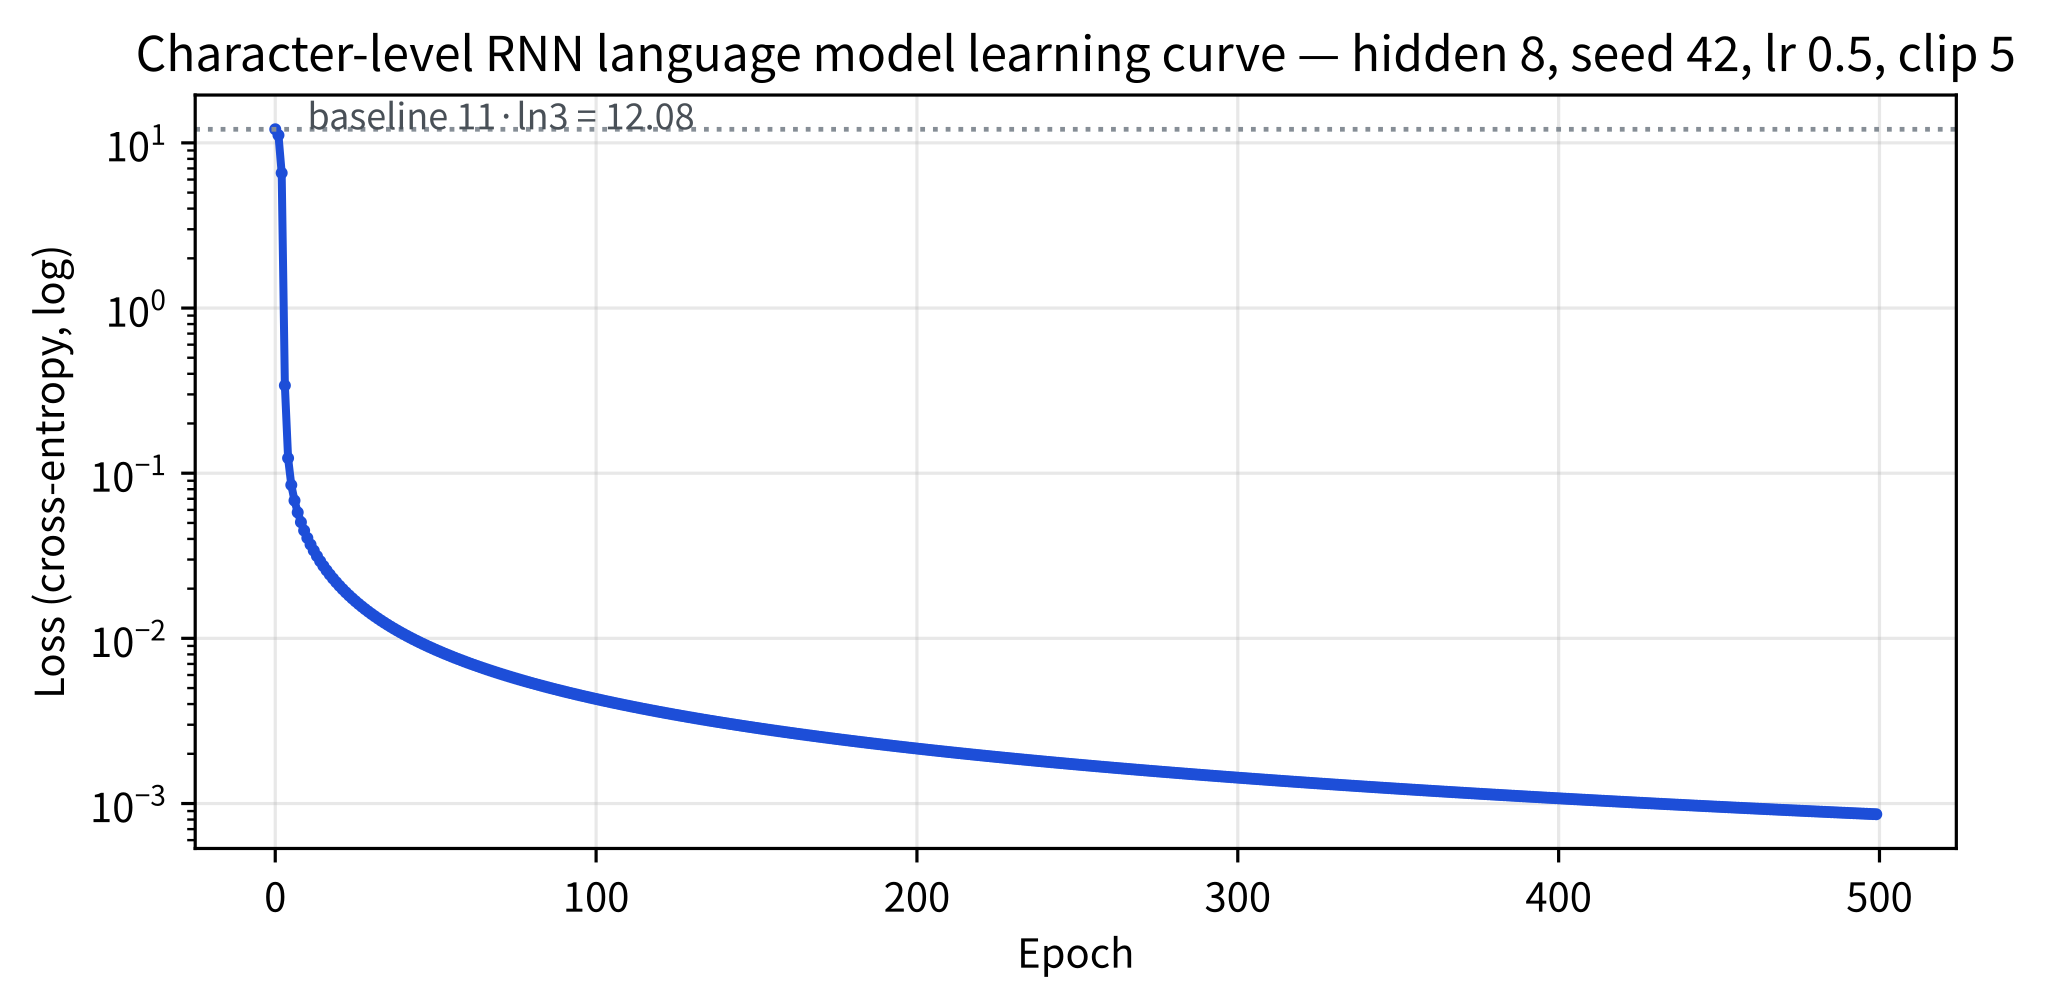
\includegraphics[width=\linewidth]{ch11_2_rnn_loss_curve.png}
      \vskip0.3em
      {\footnotesize 초기 12.09 $\to$ 10에폭 0.045 $\to$ 500에폭
      0.0009 (로그 스케일).}
    \end{column}
  \end{columns}
\end{frame}

\begin{frame}{손실 곡선이 보여주는 것: 한 번에 모든 시점}
  \begin{itemize}
    \item BPTT가 ``시점 11곳의 오차를 \textbf{전부 모아} 시간을
      거슬러 전달''하기 때문에
    \item \textbf{한 번의 에폭마다 모든 시점의 예측이 \textbf{동시에}
      개선}된다
    \item 시점마다 \textbf{독립적으로} 학습했다면 이렇게 가파르게
      떨어지지 않았을 것
  \end{itemize}
  \vskip0.6em
  \begin{block}{왜 시점마다 따로 학습하면 안 되나}
    각 시점의 예측이 그 이전 시점들에 어떻게 의존하는지(BPTT가
    계산하는 바로 그 의존성)를 전혀 반영하지 못한다. ``다음 문자를
    맞히는 능력''은 결국 ``이전 문자들을 \textbf{얼마나 잘
    요약했는가}''에 달려 --- 손실을 전체 시퀀스에 대해 계산하고
    역전파도 시간을 거슬러 전체에 해야 \textbf{은닉 상태가 실제로
    유용한 요약을 배우게} 된다.
  \end{block}
\end{frame}

\begin{frame}{자주 하는 실수: 그래디언트 클리핑을 빼먹는 것}
  학습 코드에 \verb|np.clip(dP, -5, 5)|로 그래디언트를 일정 범위로
  \textbf{잘라내는(clipping)} 단계가 있다 --- 이걸 빼먹으면?
  \begin{itemize}
    \item 그래디언트는 시점을 거슬러 내려올 때마다
      $W_{hh}^\top \tanh'$를 계속 곱함
    \item 학습 초반 가중치가 아직 ``좋지 않은'' 상태일 때 이 곱적이
      1보다 커질 수 있음 $\Rightarrow$ 그래디언트가
      \textbf{지수적으로 커져} 손실이 갑자기 \textbf{튀거나
      NaN}이 됨
  \end{itemize}
  \vskip0.5em
  \begin{block}{이 예제의 정량적 실측}
    학습률 2.0, 클리핑 \textbf{끄고} 500 에폭: 세 가중치 행렬의
    절대값 최댓값 합 $\approx$ \textbf{47만} (467,172).\\
    같은 설정으로 클리핑(상한 5) \textbf{켜면}: $\approx$ \textbf{83}
    에 멈춤 --- \textbf{약 5,600배 차이}.
  \end{block}
  \vskip0.4em
  {\footnotesize Ch.\,2.1의 학습률 발산과 원인은 다르다(학습률이
  아니라 \textbf{시퀀스 길이에 걸친 곱셈}이 원인) --- 증상은 똑같다.
  손실이 갑자기 NaN이 되면 \textbf{그래디언트 폭발부터 의심}하고,
  클리핑이나 더 작은 학습률을 먼저 시도 --- RNN 계열 디버깅의
  첫 단계.}
\end{frame}

\begin{frame}{자주 하는 실수: \verb|+=|을 \verb|=|로 쓰는 것}
  \begin{itemize}
    \item \textbf{더 흔한} 실수: BPTT 루프에서 \verb|dWhh += ...|를
      \verb|dWhh = ...|로 쓰는 것
    \item $W_{hh}$가 모든 시점에서 공유되므로 각 시점의 기여를
      \textbf{더해야} 하는데, \verb|=|로 쓰면
      \textbf{가장 마지막(가장 과거) 시점 기여 하나만 남고} 나머지가
      \textbf{덮어쓰임}
    \item 증상: ``학습은 되는데 \textbf{느리고}, 긴 시퀀스일수록 더
      못 배운다'' --- \textbf{손실을 한 시점만} 보고 있는 것과
      같으니까
  \end{itemize}
  \vskip0.6em
  \begin{block}{BPTT 코드를 읽을 때 \textbf{첫째로} 확인할 두 줄}
    (1) \textbf{그래디언트 클리핑}이 있는가?
    \\ (2) \verb|dWhh +=| 가 \verb|dWhh =|가 아닌가?
  \end{block}
\end{frame}

\begin{frame}{실전: 잘라내기 BPTT (truncated BPTT)}
  실제로 긴 문장을 학습할 때 $T$가 커지면:
  \begin{enumerate}
    \item 그래디언트 곱적이 지수적으로 소실 $\Rightarrow$
      \textbf{먼 과거가 거의 학습에 기여하지 못}함
    \item 계산·메모리가 $T$에 \textbf{비례}해 증가
  \end{enumerate}
  $\Rightarrow$ 시퀀스를 \textbf{여러 개의 짧은 창(window)으로
  잘라} 각 창별로 BPTT를 하고, \textbf{은닉 상태만 창 사이로
  넘겨주는} 잘라내기 BPTT.
  \begin{itemize}
    \item ``창 길이''는 \textbf{소실되는 신호와 계산량} 사이의
      하이퍼파라미터
    \item \kq{LSTM은(11.3절) 이 잘라내기에 크게 의존하지 않도록
      \textbf{그래디언트 경로 자체}를 수정한 구조임을 대비해서
      기억.}
  \end{itemize}
\end{frame}

\begin{frame}{잘라내기가 ``거의 같은'' 이유}
  \begin{itemize}
    \item 잘라내기가 ``약한'' 것이 아니라 ``\textbf{거의 같은}''
      이유: \textbf{곱적이 지수적으로 소실되기 때문}
    \item 초기(학습 전) 가중치에서: 전체 11시점 BPTT로 구한
      $W_{hh}$ 그래디언트 노름 $\gg$ 마지막 4시점만 BPTT로 구한
      것 --- 그러나 \textbf{그 차이가 생각만큼 크지 않음}
    \item 먼 과거(시점 1$\sim$7)의 기여는 $W_{hh}^\top$을 \textbf{여덟
      번 곱한 곱적}이라 이미 많이 작아져, \textbf{4시점 창으로
      잘라도 전체 그래디언트의 상당 부분이 재현}
    \item 300에폭 진행 시 \textbf{전체 BPTT든 창 길이 4든}
      ``abcabcabcabc''를 정확히 재현
  \end{itemize}
  \vskip0.5em
  \begin{block}{의의}
    긴 시퀀스에서 ``\textbf{먼 과거의 그래디언트}''는 본질적으로
    \textbf{미미}하므로 잘라내기의 \textbf{비용은 생각보다 작다}.
  \end{block}
\end{frame}

\begin{frame}{FAQ: 에폭이 많은 이유, $W_{hh}$ 미분}
  \begin{block}{Q. 왜 이렇게 많은 에폭이 필요했나요?}
    일부러 아주 단순한 구조(은닉 8)와 \textbf{기본 경사하강법}
    (Adam이 아니라)으로 \textbf{손으로 따라가기 쉽게} 만들었기
    때문 --- 실전에서는 Adam(Chapter 9의 SGD를 개선한 옵티마이저)
    + 더 큰 은닉 크기로 훨씬 적은 반복에 수렴.
    \kq{중요한 것은 몇 에폭이 걸렸는가가 아니라, 손실이 실제로
    0에 가깝게(12.09 $\to$ 0.00086) 줄었고 생성 문자열이 정답과
    일치했다는 사실 자체.}
  \end{block}
  \vskip0.6em
  \begin{block}{Q. $W_{hh}$가 공유되니까 BPTT에서 ``한 번만'' 미분하면
  안 되나요?}
    아니다 --- \textbf{미분은 각 시점에서 각각} 해야 하고, 그
    결과를 같은 $W_{hh}$의 그래디언트 텐서에 \textbf{더해야} 함
    (\verb|+=|).
    \begin{itemize}
      \item 공유된 파라미터의 그래디언트 = 계산 그래프에서
        \textbf{그 파라미터가 몇 번 쓰였는지만큼}의 기여 합
      \item CNN의 필터(Ch.\,10)도 같은 원리: 하나의 필터가 이미지
        위에 $n^2$번 쓰이면 그 필터의 그래디언트는 $n^2$개 위치의
        \textbf{기여 합}
    \end{itemize}
  \end{block}
\end{frame}

\begin{frame}{확인 문제: 숫자 세 개}
  \begin{enumerate}
    \item \kb{초기 손실} --- 어휘 3문자의 이 언어모델에서, 무작위
      초기화($\approx$ 균등 분포)의 초기 손실을 ``시점 수 $\times$
      $\log V$''로 예상하라. 12문자 시퀀스(11개 예측)라면
      \textbf{얼마인가}? ($11 \times \log 3$) 이 ``기준선''을
      아는 것이 왜 중요한지 한 문장으로.
    \item \kb{그래디언트 누적} --- 손계산 예제의
      $\frac{\partial L}{\partial W_{hh}} = \begin{bmatrix}
      0.1000 & 0.1587 \\ -0.0365 & -0.0579 \end{bmatrix}$ 이 값이
      \textbf{두 시점의 기여 합}임을 유도 식 $(A)+(B)$로 설명.
      \verb|dWhh = ...|(대입)를 썼다면 어떤 값만 남았을지 추정.
    \item \kb{곱적의 양} --- $\tanh'(z) \approx 0.5$, $W_{hh}$ 크기
      1.2일 때, $T=20$이면 $\prod_{t=2}^{20} (0.5 \times 1.2)$는
      \textbf{몇 배}? ($0.6^{20} \approx 3.7 \times 10^{-5}$)
      소실인지 폭발인지, 왜 그런지 한 문장으로.
  \end{enumerate}
\end{frame}

% ============================================================
\section{11.3 그래디언트 소실의 재발과 LSTM/GRU}

\begin{frame}{그래디언트 소실이 시간 축에서 재발}
  Ch.\,9.2에서 본 것과 \textbf{정확히 같은 패턴}:
  \begin{itemize}
    \item $\tanh'$의 최댓값은 1이지만 \textbf{대부분의 구간에서 1보다
      작}고
    \item 여기에 $W_{hh}$까지 $T$번(시퀀스 길이만큼) 곱해진다
    \item 시퀀스가 길수록($T$가 클수록) 이 곱은
    \begin{itemize}
      \item $W_{hh}$ 고유값 $< 1$: 지수적으로 0에 가까워짐
        --- \kb{그래디언트 소실}
      \item $W_{hh}$ 고유값 $> 1$: \textbf{발산}
        --- \kb{그래디언트 폭발}
    \end{itemize}
  \end{itemize}
  \vskip0.5em
  \begin{itemize}
    \item 결과: 기본 RNN은 \textbf{먼 과거의 정보를 거의 기억하지
      못}한다 --- ``10단어 전에 나온 주어''를 지금 활용해야 하는
      문장에서 특히 취약
  \end{itemize}
  \vskip0.4em
  숫자로 ($\tanh' \approx 0.5$, $W_{hh}$ 크기 0.9, $T=20$):
  \[ (0.5 \times 0.9)^{20} = 0.45^{20} \approx 4.5 \times 10^{-7}
     \;\;(\text{사실상 0}) \]
  {\footnotesize 20단어 전의 정보는 지금 시점의 학습에 거의 아무
  영향도 주지 못한다.}
\end{frame}

\begin{frame}{``소실''이 지수함수라는 것: 표로}
  $\frac{\partial h_T}{\partial h_1} = \prod_{t=2}^{T} \tanh'(z_t)\, w_{hh}$
  (스칼라 단순화)를 $T$를 크게 올려가며 계산:
  \vskip0.4em
  \scriptsize
  \begin{tabular}{@{}l|ccc@{}}
    \toprule
    시퀀스 길이 $T$ & $\tanh'=0.5,\; w_{hh}=0.9$ (승수 0.45) &
      $w_{hh}=1.5$, 포화 $\tanh'=0.5$ (승수 0.75) &
      $w_{hh}=1.5$, 미포화 $\tanh' \approx 1$ (승수 1.5) \\
    \midrule
    5 & $0.45^{4} \approx 4.1 \times 10^{-2}$ & $0.75^{4}
      \approx 3.2 \times 10^{-1}$ & $1.5^{4} \approx 5.1$ \\
    10 & $0.45^{9} \approx 7.6 \times 10^{-4}$ & $0.75^{9}
      \approx 7.5 \times 10^{-2}$ & $1.5^{9} \approx 38$ \\
    20 & $0.45^{19} \approx 2.6 \times 10^{-7}$ & $0.75^{19}
      \approx 4.2 \times 10^{-3}$ & $1.5^{19} \approx 2.2 \times
      10^{3}$ \\
    50 & $0.45^{49} \approx 1.0 \times 10^{-17}$ & --- & --- \\
    100 & $0.45^{99} \approx 4.7 \times 10^{-35}$ & --- & --- \\
    \bottomrule
  \end{tabular}
\end{frame}

\begin{frame}{세 열을 읽으면 RNN 학습의 ``운명''}
  \begin{itemize}
    \item \kb{첫째 열 (승수 0.45 $< 1$)}: 전형적 \textbf{소실}.
      $T=50$이면 $10^{-17}$으로, \texttt{float32}의 표현 하한
      ($\sim 10^{-38}$) 근처까지 밀림 --- ``100단어 전의 주어''의
      그래디언트는 \textbf{수치적으로 0과 구별 불가능}, 그 자리의
      가중치는 \textbf{영원히 갱신되지 못}함
    \item \kb{둘째 열 (승수 0.75)}: 같은 소실이지만 \textbf{16,000배
      느리다} --- $w_{hh}$를 0.9에서 1.5로 올리자 소실은
      \textbf{사라지지 않고 속도만 줄었다}. ``게이트 없이 소실을
      극복하려 하면 \textbf{소실$\leftrightarrow$폭발 사이 줄타기}에
      불과''하다는 뜻
    \item \kb{셋째 열 (승수 1.5 $> 1$)}: \textbf{폭발}. $T=20$에서
      이미 $2.2 \times 10^{3}$, $T=50$이 넘으면 $10^{10}$ 대로
      \texttt{NaN} --- 11.2절의 \verb|np.clip| 그래디언트
      클리핑이 바로 이 열을 막기 위한 \textbf{급조된 처방}
      (Pascanu et al., 2013)
  \end{itemize}
  \vskip0.4em
  \kq{승수 1 하나를 ``조금만'' 넘기면(1에 가까이) 소실이 느려지고,
  크게 넘기면 폭발이 된다. 어떤 초기화를 잡아도 \textbf{지수함수
  라는 형 자체}는 바뀌지 않는다 --- 이 형을 바꾸는 것이 곧
  \textbf{게이트의 임무}.}
\end{frame}

\begin{frame}{소실/폭발 갈라지는 세 곡선}
  \begin{columns}[T]
    \begin{column}{0.52\textwidth}
      \centering
      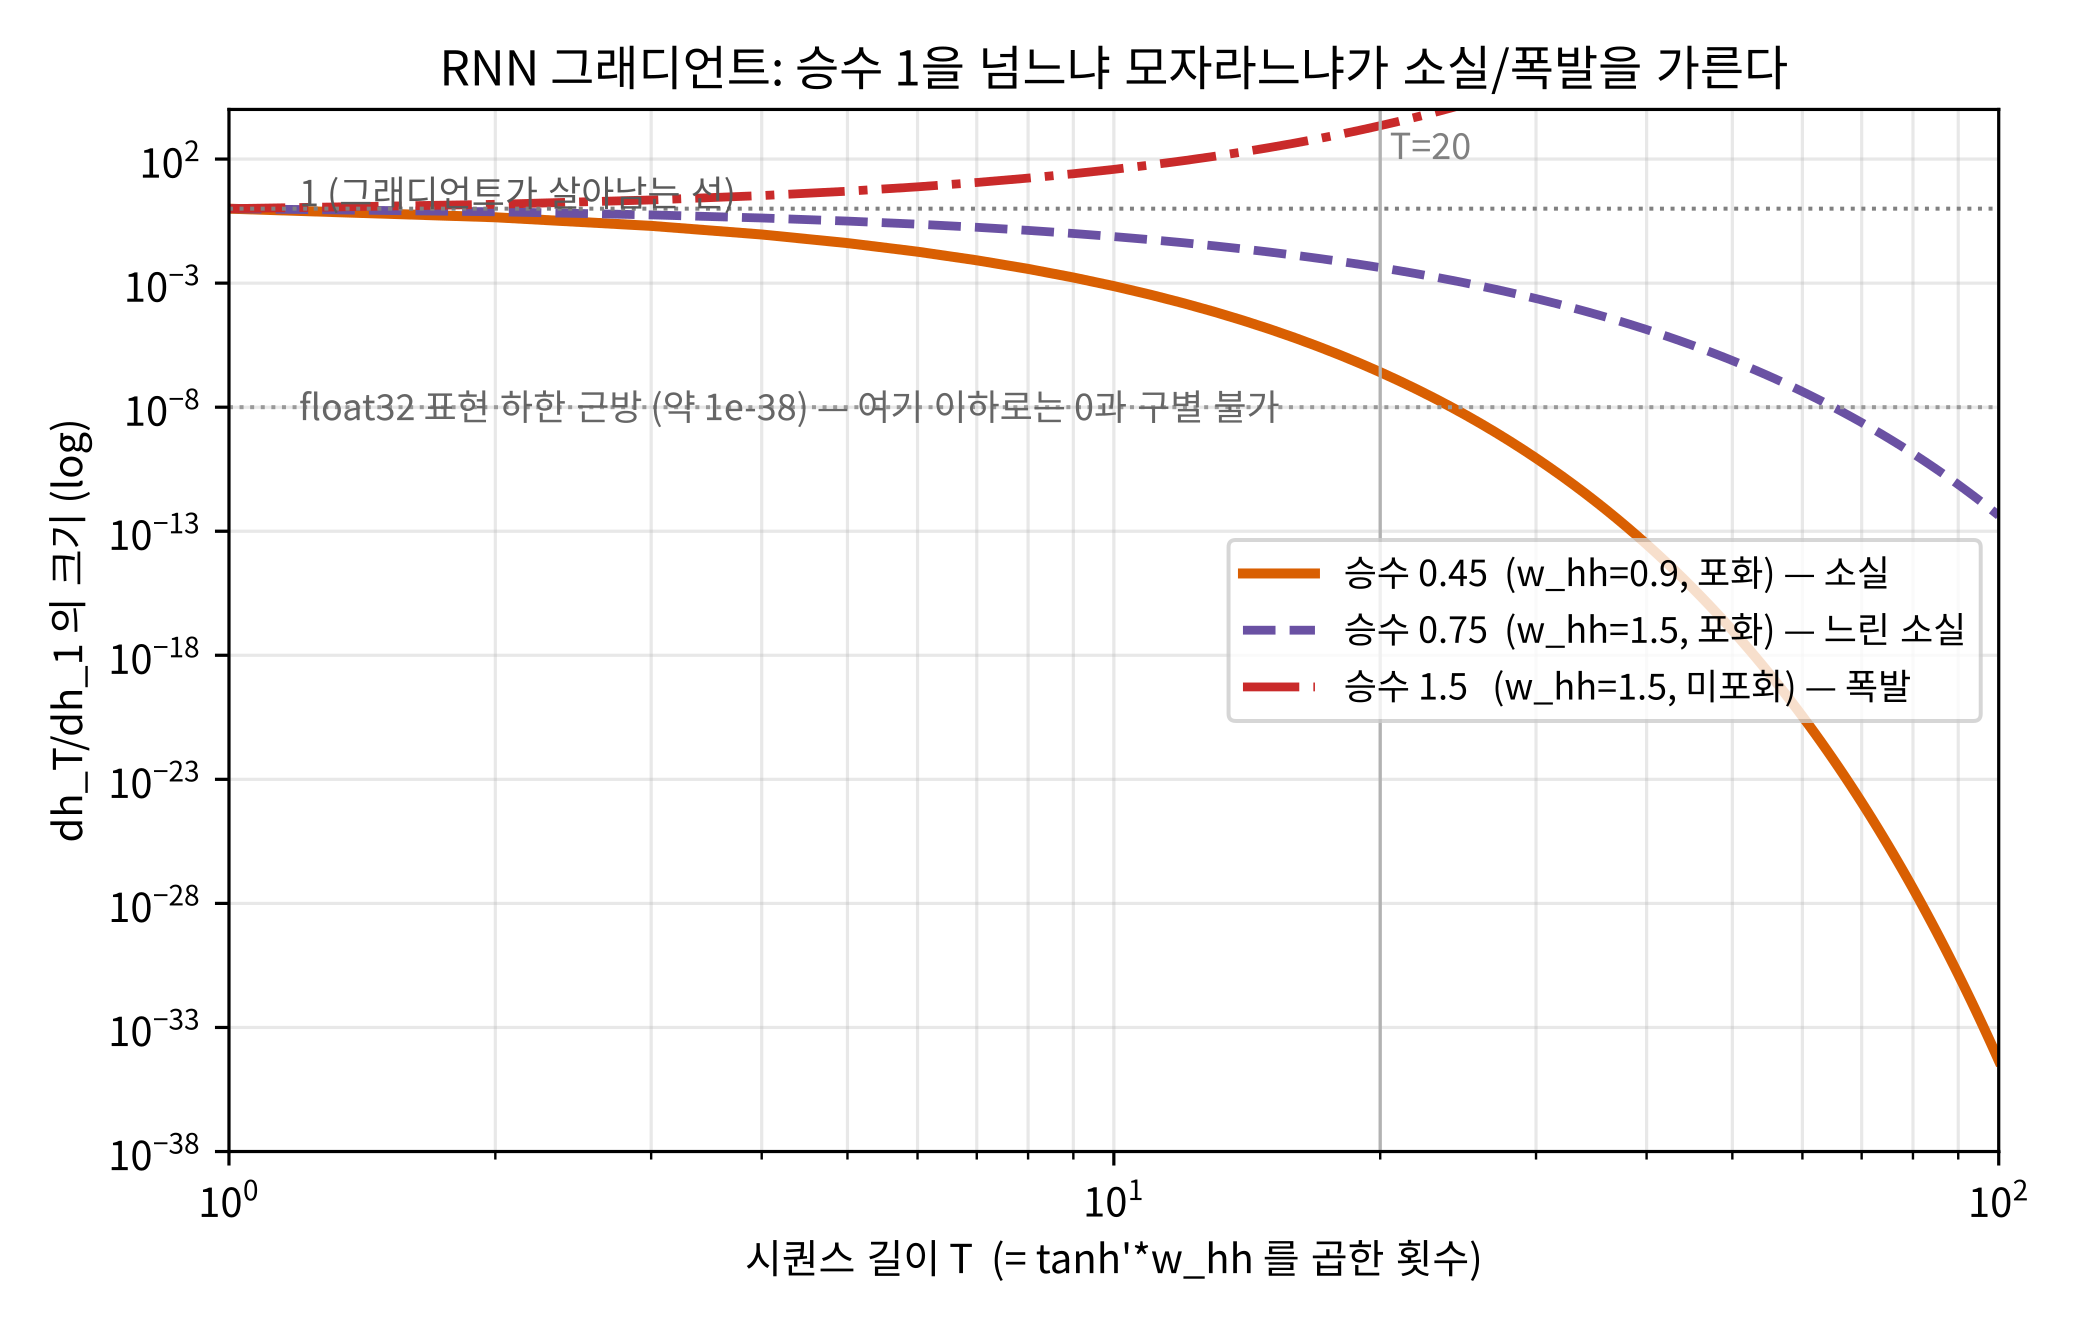
\includegraphics[width=\linewidth]{ch11_3_decay.png}
      \vskip0.3em
      {\footnotesize 승수 0.45 / 0.75 / 1.5의 그래디언트 곱이
      시퀀스 길이 $T$에 대해 지수적으로 소실 · 느린 소실 ·
      폭발로 갈라지는 곡선.}
    \end{column}
    \begin{column}{0.48\textwidth}
      \begin{block}{핵심 통찰}
        ``\textbf{승수의 밑}이 1보다 작으면 지수 소실, 크면 지수
        폭발''.
      \end{block}
      \vskip0.5em
      \begin{itemize}
        \item 초기화를 $W_{hh}$ 고유값이 1 근처에 오도록 정교하게
          맞춰야 한다는 11.2절의 ``자주 하는 실수''가 여기서 그
          \textbf{깊이}를 드러냄
        \item 그러나 어떤 초기화도 \textbf{지수}라는 형은 못 바꿈
        $\Rightarrow$ \textbf{구조}를 바꿔야 함
      \end{itemize}
    \end{column}
  \end{columns}
\end{frame}

\begin{frame}{왜 곱셈이 문제고 덧셈은 아닌가}
  ``곱을 반복하면 지수''는 수학의 당연한 결과 ($a^T$). 그런데 같은
  길이의 사슬이어도, \textbf{각 단계가 이전 값을 ``곱으로'' 이어가는지
  ``더함으로'' 이어가는지}에 따라 그래디언트의 운명이 완전히
  갈린다.
  \vskip0.5em
  \begin{columns}[T]
    \begin{column}{0.5\textwidth}
      \kb{기본 RNN (11.2절)}: 이전 은닉 상태를 \textbf{곱}해서
      전달
      \vskip0.3em
      \[ h_t = \tanh(\cdots + W_{hh}\, h_{t-1})
         \quad \Longrightarrow \quad
         \frac{\partial h_t}{\partial h_{t-1}} \propto W_{hh}
         \;\;(\text{매 단계 곱}) \]
      \vskip0.3em
      매 단계마다 그래디언트를 \textbf{할인율 $< 1$}로 곱함.
    \end{column}
    \begin{column}{0.5\textwidth}
      \kb{ResNet 스킵 연결 (Ch.\,10.2)}: \textbf{더함}
      $y = F(x) + x$
      \vskip0.3em
      \[ \frac{\partial y}{\partial x} =
         \frac{\partial F(x)}{\partial x} + 1 \]
      \vskip0.3em
      \textbf{``+1''이 매 스킵마다 정확히 1의 그래디언트를
      통과시킴} --- 미분 경로가 1로 ``단락''해 있다. 스킵 20개를
      쌓아도 $0.45^{20}$이 아니라 $(1 + 0.45)^{20} \approx
      3.7 \times 10^{2}$ --- \textbf{할인 없이 1 그대로} 한
      가닥을 통과.
    \end{column}
  \end{columns}
\end{frame}

\begin{frame}{LSTM의 ``고속도로'': ResNet 스킵의 시간 축 버전}
  \begin{itemize}
    \item LSTM/GRU가 이끄는 ``고속도로'' = \textbf{ResNet 스킵
      연결의 시간 축 버전}
    \item \kb{LSTM의 셀 상태 $C_t$}는 매 시점 ``전부 버리고 새로
      계산''하는 것이 \textbf{아니라}:
      \[ C_t = \underbrace{f_t \odot C_{t-1}}_{\text{기억 유지
         (덧셈·스킵)}} \;+\; \underbrace{i_t \odot \tilde C_t}_{\text{신규
         정보 추가 (덧셈)}} \]
    \item 이전 셀 상태에 \textbf{더해져서} 전달된다
    \item \textbf{곱셈(게이트)}은 ``얼마나 남길지''라는
      \textbf{크기 조절 스위치}로만 사용
    \item 정보 \textbf{본체}가 지나가는 통로는 \textbf{덧셈}
  \end{itemize}
  \vskip0.5em
  \kq{이 한 문장이 곧 ``왜 LSTM이 긴 시퀀스에 강한가''의
  전부 --- Ch.\,10.2 스킵 연결과 Ch.\,9.2 ``미분이 1에 가까울수록
  그래디언트가 산다''가 시간 축에서 합류한 지점.}
\end{frame}

\begin{frame}{게이트(gate): LSTM 3개, GRU 2개}
  ``게이트''는 이름만큼 단순한 장치: $\sigma(\cdot)$ 시그모이드로
  산출한 \textbf{0과 1 사이의 숫자}로, ``이 정보를 \textbf{얼마나
  통과/유지/갱신할 것인가}''를 \textbf{데이터와 학습}으로 결정하는
  \textbf{연속 스위치} (0 = 완전 차단, 1 = 완전 개방).
  \vskip0.5em
  \small
  \begin{tabular}{@{}llp{7.5cm}@{}}
    \toprule
    모델 & 게이트 & 역할(한 줄) \\
    \midrule
    LSTM & \textbf{망각 게이트} $f_t$ & ``기억(셀 상태)에서 지금
      버릴 부분은?'' --- 1이면 그대로 유지 \\
    LSTM & \textbf{입력 게이트} $i_t$ & ``지금 새로 기억에 쓸어
      넣을 정보는?'' \\
    LSTM & \textbf{출력 게이트} $o_t$ & ``저장된 기억 중 지금
      출력에 보여줄 부분은?'' \\
    GRU & \textbf{갱신 게이트} $z_t$ & 망각$+$입력을 하나로 통합:
      ``기억의 얼마나를 새 값으로 교체할지'' \\
    GRU & \textbf{출력 게이트} $r_t$ & LSTM 출력 게이트와 같은
      역할 \\
    \bottomrule
  \end{tabular}
  \vskip0.6em
  \begin{block}{공통 분모}
    \textbf{LSTM = 3개의 스위치, GRU = 2개의 스위치} --- GRU는
    LSTM의 망각·입력 게이트를 하나의 ``갱신'' 결정으로 \textbf{합쳐}
    파라미터를 줄였다. RNN의 ``은닉 상태 \textbf{전체}를 매번 새로
    쓴다''를, 게이트는 ``\textbf{어떤 부분은 보존하고 어떤 부분만
    바꾸라}''고 학습된 판단을 내리게 만든다. 공통 원리: \textbf{곱}으로
    조절하는 \textbf{스위치} + \textbf{덧}으로 전달하는 \textbf{통로}.
  \end{block}
  {\footnotesize 자세한 게이트 수식은 이번 학기에서는 다루지
  않는다.}
\end{frame}

\begin{frame}{LSTM 셀: 곱은 스위치, 덧셈은 고속도로}
  \begin{columns}[T]
    \begin{column}{0.55\textwidth}
      \centering
      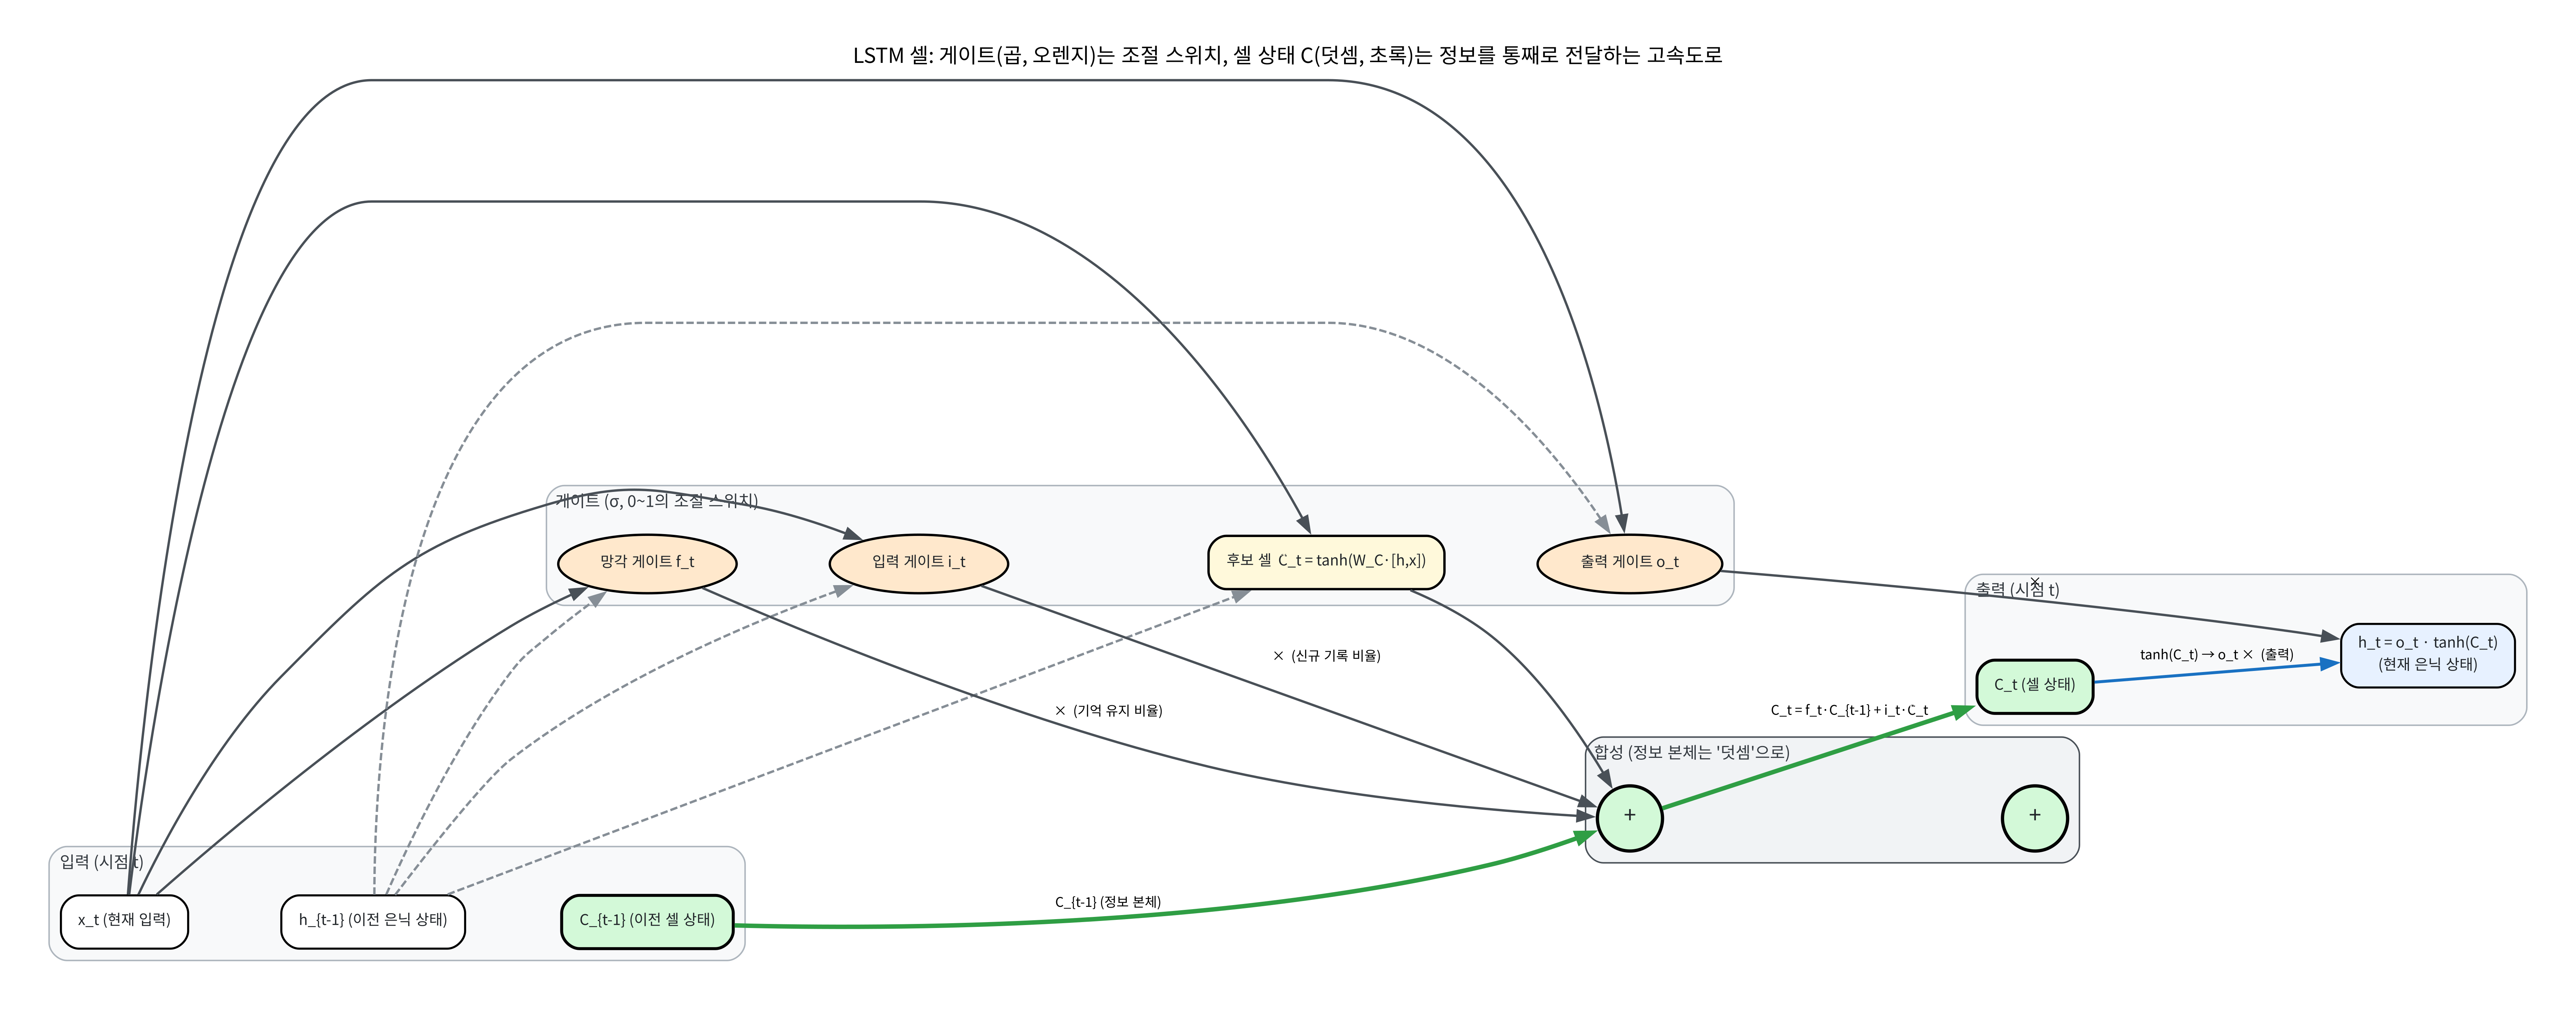
\includegraphics[width=\linewidth]{ch11_3_lstm_cell.png}
    \end{column}
    \begin{column}{0.45\textwidth}
      이전 셀 상태 $C_{t-1}$이 \textbf{망각 게이트 $f_t$와
      곱해지고}(조절), \textbf{입력 게이트 $i_t \cdot \tilde C_t$가
      더해져서}(통로) $C_t$로 이어지는 구조.
      \vskip0.5em
      \begin{itemize}
        \item \kb{곱}(게이트) = ``얼마나 남길지'' 조절
        \item \kb{덧셈} = 정보가 \textbf{통째로} 지나가는
          고속도로
      \end{itemize}
      \vskip0.5em
      \kq{이 분리(조절/통로)가 기본 RNN의 ``전체 갱신(곱만)''과
      구별되는 전부.}
    \end{column}
  \end{columns}
\end{frame}

\begin{frame}{셀 상태의 그래디언트가 왜 1 근처를 유지하는가}
  ``셀 상태가 덧셈으로 전달된다''를 그래디언트 관점에서 정확히
  전개. 게이트만 추상화하면:
  \vskip0.4em
  \[ C_t = \underbrace{f_t \cdot C_{t-1}}_{\text{기억 유지}}
     \;+\; \underbrace{i_t \cdot \tilde C_t}_{\text{신규 기록}}
     \qquad (f_t, i_t \in (0,1)) \]
  \vskip0.4em
  기억이 시점 1에서 $T$까지 전해지는 그래디언트: 신규 기록 항
  ($i_t \tilde C_t$)은 $C_{t-1}$에 무관하므로 미분에서 \textbf{떨어져
  나가고},
  \vskip0.4em
  \[ \frac{\partial C_T}{\partial C_1} = \prod_{t=2}^{T} f_t \]
  \vskip0.4em
  \begin{itemize}
    \item \kb{RNN의 $\prod \tanh'(z_t)\, w_{hh}$에서 $\tanh'$
      (고정 할인율, $\approx 0.45$)의 자리에 \textbf{학습된
      망각 게이트 $f_t$}가 들어온 것}
  \end{itemize}
\end{frame}

\begin{frame}{차이 두 가지: 1에 수렴 + 통로 오염 없음}
  \begin{enumerate}
    \item \kb{곱해질 수 있는 게 0$\sim$1이 아니라 (학습으로) 1에
      수렴할 수 있다} --- 기본 RNN의 승수 0.45는 \textbf{구조가}
      1 미만으로 \textbf{고정}이지만, ``계속 기억해야 한다''는 패턴을
      학습하면 망각 게이트가 \textbf{1에 가깝게 수렴} (이상적 해답
      $f_t = 1$)
    \item \kb{덧셈 항이 ``기억 통로''를 오염시키지 않는다} ---
      $i_t \tilde C_t$는 그래디언트를 \textbf{생성}하지만 기존
      $C_{t-1}$이 통과하는 경로를 \textbf{할인하지는 않}는다
  \end{enumerate}
  \vskip0.5em
  게이트가 $f_t \approx 0.99$로 학습되면 $T=100$에서
  $0.99^{99} \approx 0.37$ vs RNN $0.45^{99} \approx 4.7 \times
  10^{-35}$ --- \textbf{약 $10^{33}$ 배가 잘 보존}. 승수의 \textbf{밑이
  0.45에서 0.99로 이동}한 것: 아직 지수이고 1은 아니지만,
  \textbf{학습이 그 밑을 문제의 필요에 맞게 밀어 올릴 수 있는
  것}.
  \vskip0.4em
  \kq{단, 게이트가 \textbf{있어}서가 아니라 게이트가 \textbf{1에
  수렴할 때} 기억이 사는 것 (아래 ``기억 과제'' 실험이 보여줌).}
\end{frame}

\begin{frame}{게이트의 비용: 파라미터가 얼마나 늘까}
  게이트는 \textbf{공짜가 아니다}. 기본 RNN은 시점마다
  $W_{xh}, W_{hh}, W_{hy}$ 세 개($\approx 2\,d_{in}d_h + d_h^2$)인데,
  게이트 모델은 \textbf{이 조합을 3$\sim$4개로 복제}.
  \vskip0.4em
  입력 차원 $d_{in} = 512$, 은닉 크기 $d_h = 128$에서:
  \small
  \begin{tabular}{@{}lll@{}}
    \toprule
    모델 & 시점당 가중치($\approx$) & 기본 RNN 대비 \\
    \midrule
    기본 RNN & $512 \cdot 128 + 128^2 \approx 8.2 \times 10^{4}$
      & 1$\times$ \\
    GRU (게이트 3) & $3(d_{in} + d_h)\,d_h \approx 2.5 \times
      10^{5}$ & \textbf{$\approx 3\times$} \\
    LSTM (게이트 4) & $4(d_{in} + d_h)\,d_h \approx 3.3 \times
      10^{5}$ & \textbf{$\approx 4\times$} \\
    \bottomrule
  \end{tabular}
  \vskip0.5em
  \begin{itemize}
    \item 게이트 하나마다 입력$\to$은닉, 은닉$\to$은닉 가중치 한
      조($(d_{in}+d_h)\,d_h$) 추가
    \item LSTM $\approx$ 4배, GRU $\approx$ 3배의 \textbf{메모리·계산}
    \item \kq{\textbf{데이터가 적은 문제에서는 게이트 모델이 오히려
      과적합}하기 쉬움 --- ``파라미터를 더 사서 버는 능력''과 ``더
      사서 무너지는'' 사이에 Ch.\,6의 \textbf{편향-분산 트레이드오프}
      가 그대로 놓여 있다.} 게이트가 \textbf{시퀀스가 충분히 길어
      소실이 실제로 병이 될 때}에 비로소 3$\sim$4배의 비용이
      \textbf{값}을 하는 것이다.
  \end{itemize}
\end{frame}

\begin{frame}{역사: 1997년에 이미 알고 있었지만 생태계는 20년 뒤에
왔다}
  이 문제는 \textbf{새롭지 않다} --- 시그모이드/타인 망의 그래디언트
  소실은 1990년대 초부터 알려져 있었고, 1997년 \kb{셉
  훙하이저}(Sepp Hochreiter)와 \kb{유르겐
  슈미트허버}(Jürgen Schmidhuber)의 \textbf{LSTM} 논문(Hochreiter
  \& Schmidhuber, 1997)은 이미 ``\textbf{곱 대신 덧셈으로 기억을
  전달하자}''는 해결책을 냈다.
  \begin{itemize}
    \item 1999$\sim$2000년대 LSTM이 기본 RNN을 압도함이 확인됐는데도
      \textbf{2010년대 중반까지 ``지나치게 복잡한 비주류 기법''으로
      방치}
    \item 방치의 이유 = Ch.\,9.2의 \textbf{생태} 문제: GPU 메모리,
      고효율 프레임워크, He/Xavier 초기화, Adam, Dropout 등이
      \textbf{없었고} 게이트를 붙인 LSTM은 \textbf{훈련 자체가
      어려웠}다
    \item \kb{2013$\sim$2014년 GPU + 프레임워크 + 초기화/옵티마이저가
      한데 모여야} LSTM이 비로소 ``\textbf{표준}''이 됨(2014년
      seq2seq 번역·음성에서 두각)
  \end{itemize}
  \vskip0.5em
  \begin{block}{교훈 --- Ch.\,9 ``깊은 망은 세 라인(활성함수·초기화·
  최적화)이 함께 풀려야 했다''와 동일}
    \textbf{좋은 아이디어(LSTM)와 그것을 쓸 수 있는 생태계는
    \textbf{동시에} 와야 한다.}
  \end{block}
\end{frame}

\begin{frame}{실습: ``기억 과제''로 게이트가 정말 기억을 살리는가}
  ``덧셈이 소실을 늦춘다''를 공짜로 믿지 말고 \textbf{실제로
  학습해서} 확증. 과제는 의도적으로 \textbf{순차 병렬화를 배제}하고
  \textbf{장기 기억만을 고립}시킨다.
  \vskip0.6em
  \begin{block}{과제}
    길이 $T=100$의 시퀀스를 만든다. \textbf{첫 번째 토큰
    ($t=1$)은 0$\sim$9의 숫자 하나}(10차원 one-hot)이고,
    \textbf{나머지 99개 토큰은 전부 0}. 모델은 \textbf{마지막 시점
    ($t=100$)의 은닉 상태에서 ``첫 번째 토큰이 뭐였는지''}를
    분류.
  \end{block}
  \vskip0.6em
  \begin{itemize}
    \item \textbf{중간 토큰에 새 정보가 전혀 없음} --- $t=100$의
      답은 $t=1$의 정보를 \textbf{99단계에 걸쳐 그대로 운반}할 수
      있는가에 달려
    \item 기본 RNN: $0.45^{99}$ 수준의 소실로 이 ``운반''을 거의
      못 함
    \item 게이트 모델: 셀/은닉 스킵으로 정보를 \textbf{통째로
      옮겨야} 함
    \item 세 모델, \textbf{같은 은닉 크기 32, Adam, 300에폭,
      3개 seed 평균}
  \end{itemize}
\end{frame}

\begin{frame}{기억 과제: 결과}
  \small
  \begin{tabular}{@{}lcccc@{}}
    \toprule
    모델 & seed 0 & seed 1 & seed 2 & \textbf{평균} \\
    \midrule
    기본 RNN & 0.87 & 0.91 & 0.89 & \textbf{0.89} \\
    GRU & 1.00 & 1.00 & 0.98 & \textbf{0.99} \\
    LSTM & 0.61 & 1.00 & 0.96 & \textbf{0.86} \\
    \bottomrule
  \end{tabular}
  \vskip0.6em
  \begin{columns}[T]
    \begin{column}{0.55\textwidth}
      \centering
      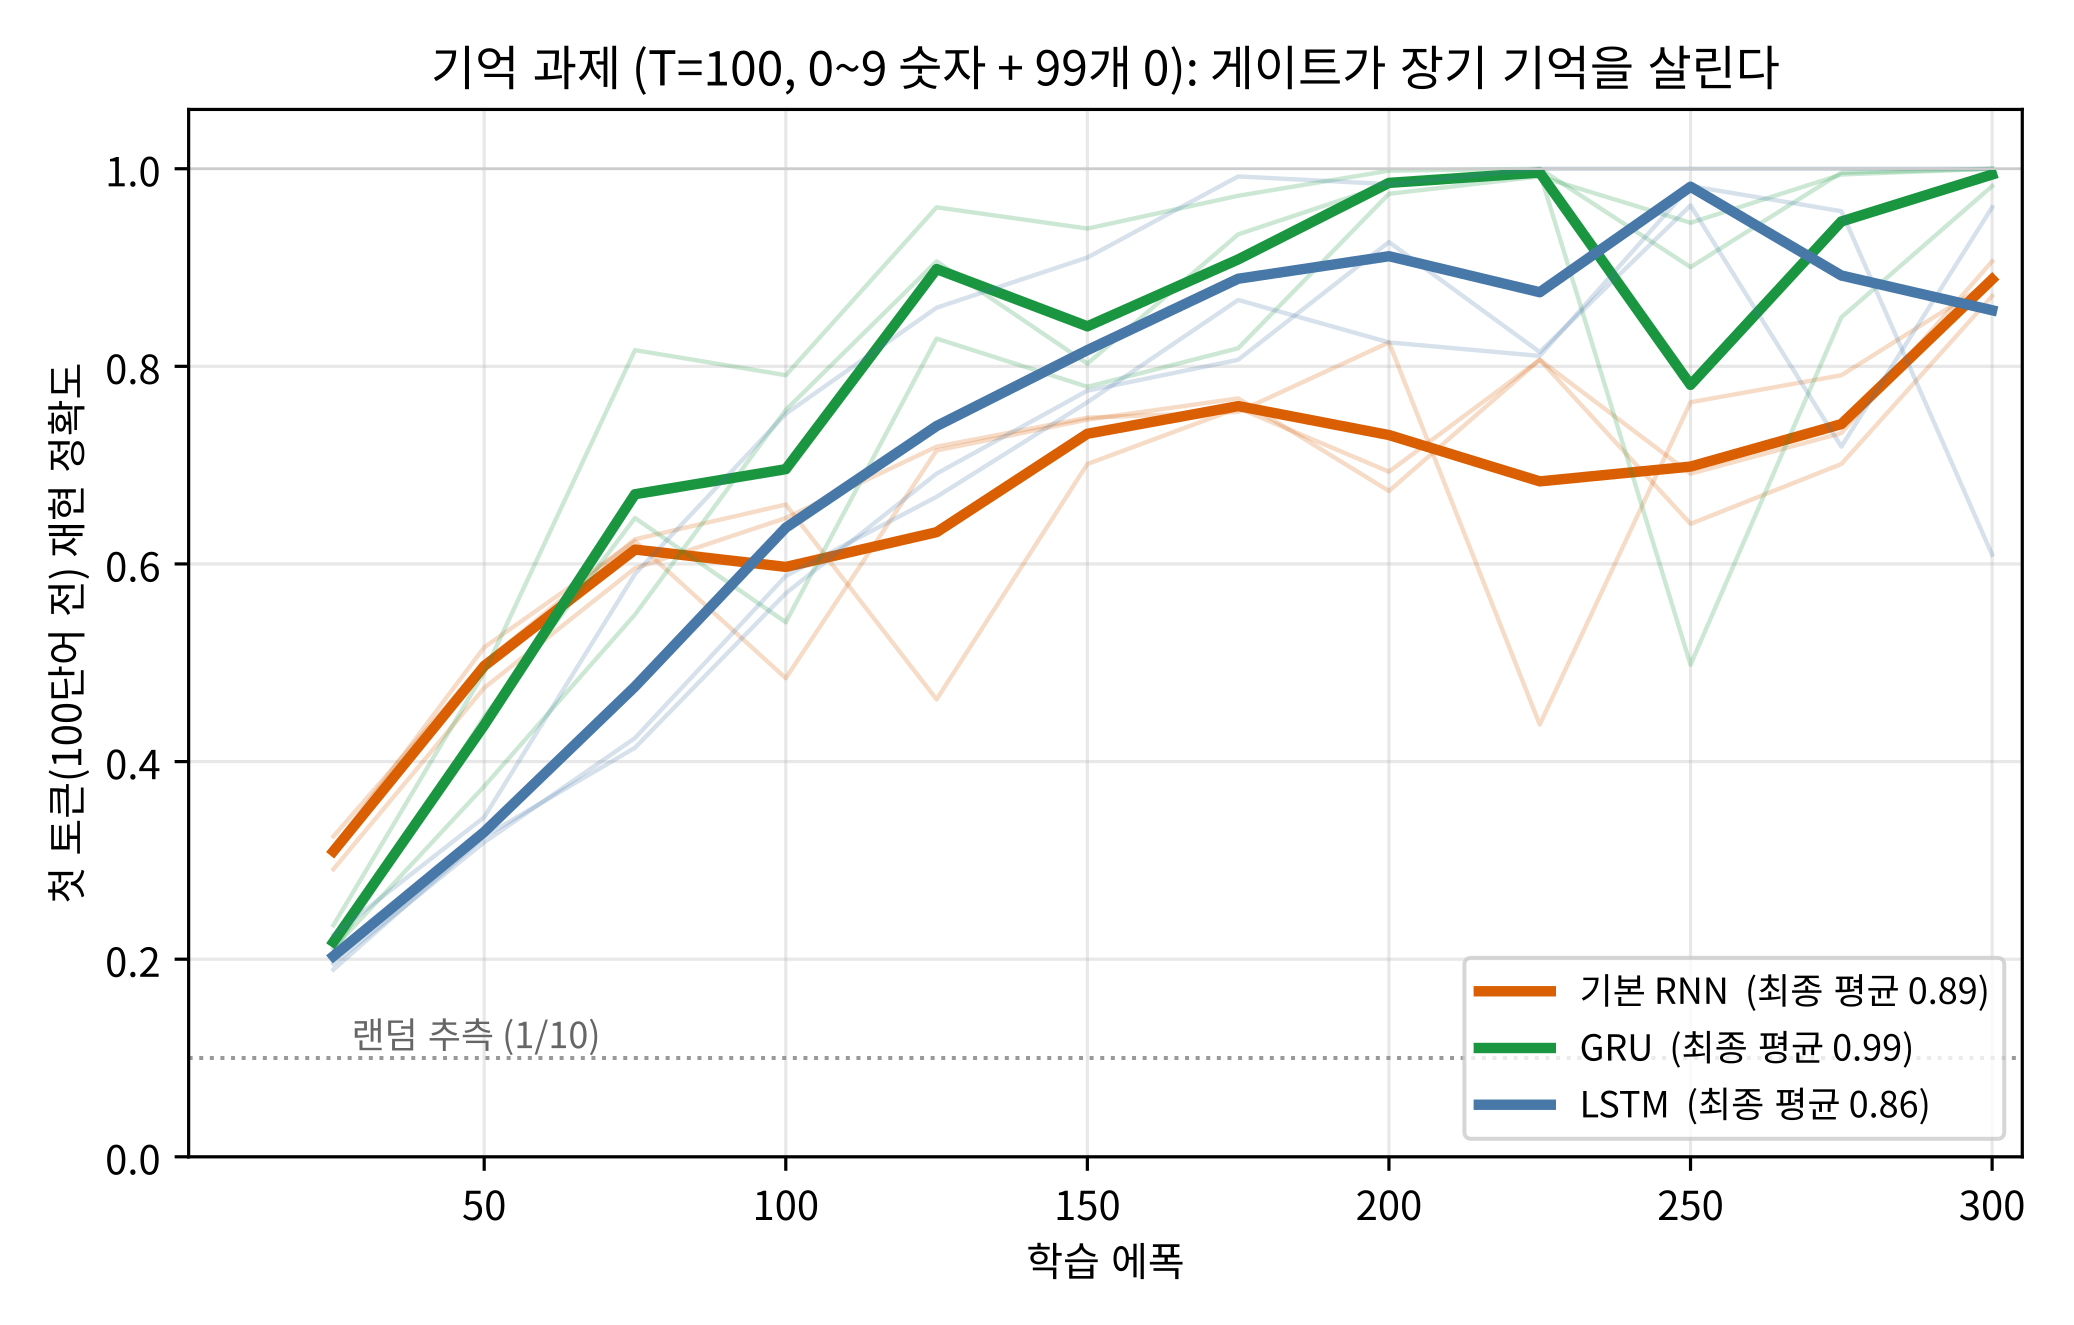
\includegraphics[width=\linewidth]{ch11_3_memory.png}
      \vskip0.3em
      {\footnotesize 기본 RNN은 0.89에 못 미치거나 흔들리고,
      GRU/LSTM은 1.00에 도달.}
    \end{column}
    \begin{column}{0.45\textwidth}
      {\footnotesize 3개 모델 $\times$ 3 seed는 CPU에서 약
      1$\sim$2분. (수식·코드는 실습 노트북 ``기억 과제'' 셀에서
      그대로 실행.)}
    \end{column}
  \end{columns}
\end{frame}

\begin{frame}{기억 과제에서 읽어야 할 세 가지}
  \begin{enumerate}
    \item \kb{게이트가 기억을 살린다}
      기본 RNN(0.89)은 ``100단어 전의 첫 단어를 맞혀라''에서 약
      10\%를 \textbf{꾸준히 놓침}. GRU(0.99)/LSTM(0.86)은 확실히
      더 높음 --- \textbf{곱을 덧셈 스킵으로 바꾼 것이 실측으로
      확인}.
    \item \kb{흥미로운 반전: GRU(0.99)가 LSTM(0.86)보다 높다}
      게이트가 \textbf{많을수록 좋은 것은 아님}. 이 과제는 데이터가
      적고(512문장) 구조가 단순해서, 파라미터가 더 많은 LSTM
      ($\approx 4\times$)이 오히려 \textbf{과적합 --- seed 간
      변동이 큼}(0.61$\sim$1.00), GRU($\approx 3\times$)가
      \textbf{더 안정적·정확} --- 아래 FAQ ``게이트가 더 적은
      GRU가 더 나은 경우가 많다''의 \textbf{생생한 증거}, Ch.\,6의
      \textbf{편향-분산 트레이드오프}가 시퀀스 모델에도 그대로
      작동.
    \item \kb{seed에 크게 흔들린다}
      LSTM의 seed 0(0.61)은 실패에 가까움. 장기 기억 같은
      ``\textbf{좁은 관}''을 통과해야 하는 학습은 \textbf{초기화에
      민감} --- \textbf{단일 실행의 숫자가 아니라 여러 seed의
      평균}을 보고 우열을 판단.
  \end{enumerate}
\end{frame}

\begin{frame}{LSTM/GRU: 게이트로 소실을 완화 --- 원리 한 줄}
  \kb{LSTM}(Long Short-Term Memory)과 \kb{GRU}(Gated Recurrent
  Unit)는 ``게이트'' 장치를 추가해, 은닉 상태를 매 시점
  \textbf{완전히 새로 계산}하는 대신 \textbf{선택적으로 유지하거나
  갱신}한다.
  \vskip0.6em
  \begin{block}{핵심 트릭}
    정보가 지나가는 경로에 \textbf{곱셈 대신 덧셈}이 섞이도록
    설계 --- Ch.\,10.2에서 본 \textbf{ResNet의 스킵 연결
    ($y = F(x) + x$)과 정확히 같은 원리}.
    \\ 덧셈은 그래디언트를 \textbf{그대로 통과}시키므로(미분이 1),
    곱셈만 반복될 때보다 \textbf{소실이 훨씬 덜}하다.
  \end{block}
  \vskip0.6em
  {\footnotesize 자세한 게이트 수식은 이번 학기에서는 다루지
  않으나, ``왜 LSTM/GRU가 기본 RNN보다 긴 시퀀스에 강한가''의
  답은 항상 이 \textbf{원리}로 귀결된다.}
\end{frame}

\begin{frame}{RNN의 근본적 한계: 순차성}
  \begin{itemize}
    \item 게이트를 추가해도 RNN은 여전히 \textbf{순차적으로 한
      시점씩} 처리해야 한다 --- 100번째 단어를 처리하려면
      1번째부터 99번째까지 \textbf{순서대로 다 거쳐}야 함
    \item 이 \textbf{순차성} 때문에:
    \begin{itemize}
      \item \textbf{병렬화가 어려}움
      \item 아주 긴 시퀀스에서는 \textbf{여전히} 먼 과거 정보가
        흐려진다
    \end{itemize}
  \end{itemize}
  \vskip0.6em
  \begin{block}{다음 장으로}
    Ch.\,12의 \kb{Attention/Transformer}는 이 \textbf{순차성 자체를
    없애는} 완전히 다른 접근이다 --- ``필요할 때마다 과거 전체를
    직접 다시 들여다본다''.
  \end{block}
  \vskip0.5em
  \kq{RNN은 ``순서가 있는 데이터를 다루려면 과거를 기억하는
  상태가 필요하다''는 통찰의 \textbf{가장 단순한 구현}이다 ---
  다음 장은 이 구조의 한계를 극복하는 이야기다.}
\end{frame}

\begin{frame}{실무 노트: 모델 고르는 ``사다리''}
  앞의 논리를 한 문장으로 실무 지침으로:
  \vskip0.6em
  \begin{center}
    \small
    기본 RNN $\to$ (길이에 따라 정확도 갈리면) \textbf{GRU} $\to$
    (여전히 부족하면) \textbf{LSTM} $\to$ (길이 극단적)
    \textbf{Attention} (Ch.\,12)
  \end{center}
  \vskip0.6em
  \begin{itemize}
    \item \kb{그래디언트 클리핑은 기본 세팅이다} --- 게이트가 소실을
      \textbf{완화}해도 \textbf{폭발}은 막아주지 않음(승수가 1을
      넘는 경로는 여전히 존재) --- 매 스텝 그래디언트 노름을 상수로
      잘라내는 클리핑은 RNN/LSTM/GRU 훈련의 \textbf{의무}
    \item \kb{망각 게이트의 ``기억하는 쪽''으로의 편향} --- 이상적
      기억 과제에서 망각 게이트는 \textbf{1(전부 유지)에 수렴}해야
      함. 게이트가 0.5 근처에서 떠돌면 ``기억을 못 한다'' 증상 ---
      \textbf{게이트의 초기화 + 초기 망각 게이트 바이어스}로 조절
      하는 것이 실전 LSTM의 잘 알려진 트릭 (Jozefowicz et al.,
      2016) --- ``게이트가 1 근처로 \textbf{초기화}되어 있어야
      기억을 \textbf{살릴 기회}가 있다''는 직감만 기억할 것
  \end{itemize}
\end{frame}

\begin{frame}{실무 노트: 과적합 감시}
  \begin{itemize}
    \item \kb{3$\sim$4배의 파라미터는 작은 데이터에서 과적합으로
      돌아온다}
    \item \textbf{train $\gg$ val gap}가 \textbf{시퀀스 길이에
      비례해 벌어진다면}:
    \begin{itemize}
      \item 모델 크기를 \textbf{줄이}거나(GRU $\to$ RNN으로 한
        칸)
      \item \textbf{dropout / early stopping}을 더 쓰는 쪽이
      \textbf{게이트를 더 붙이는 것보다 먼저} 시도해야 함
    \end{itemize}
  \end{itemize}
  \vskip0.6em
  \begin{block}{자주 하는 실수: ``소실을 완화했다''고 긴 시퀀스를
  \textbf{무조건 RNN으로}}
    게이트가 소실을 \textbf{느리게} 한다고 해서 \textbf{아무 길이든}
    LSTM/GRU가 ``기억한다''고 믿는 것은 실수. 두 가지 함정:
    \begin{itemize}
      \item \textbf{아직도 지수다, 다만 밑이 1에 가까워졌을 뿐} ---
        수천 토큰 이상이면 \textbf{LSTM/GRU도} 먼 과거를 서서히
        잃어감. ``완화이지 \textbf{해결이 아니다}'' --- 길이가
        극단적일 때는 \textbf{Attention}으로 가는 게 정답
      \item \textbf{과적합} --- 수천 문장 이하의 작은 문제에서
        ``시퀀스가 짧아 소실이 안 생길 것 같은데'' LSTM을 올리면,
        소실은 안 생기고 \textbf{과적합만} 생김 --- ``소실
        증상''(훈련 중에도 긴 시퀀스 정확도가 안 옴)과
        ``과적합 증상''(train $\gg$ val)을 구분할 줄 알아야
      한다
    \end{itemize}
  \end{block}
\end{frame}

\begin{frame}{FAQ: 완화인가, 해결인가, GRU는 못나나, 셀 vs 은닉}
  \begin{block}{Q. LSTM/GRU를 쓰면 그래디언트 소실이 완전히
  사라지나요?}
    \textbf{아니다} --- ``\textbf{완화}이지 ``해결''이 아니다.
    게이트가 곱셈 경로 옆에 \textbf{덧셈 경로}를 추가해서 소실
    속도를 크게 늦추지만, \textbf{수천 토큰 이상}이면 LSTM/GRU도
    여전히 먼 과거 정보를 점점 잃어감.
    \kq{Ch.\,12 Attention이 ``순차적으로 압축해서 기억한다''는
    접근 자체를 버리고 ``필요할 때마다 과거 전체를 직접 다시
    들여다본다''로 전환하는 이유가 바로 이것.}
  \end{block}
  \vskip0.5em
  \begin{block}{Q. GRU는 LSTM보다 항상 나쁜가요(게이트가 더 적으니까)?}
    \textbf{아니다} --- 파라미터가 적어(게이트 3개 대신 2개)
    \textbf{학습이 빠르고 데이터가 적을 때 과적합 위험도 낮음}.
    성능은 문제에 따라 둘 중 어느 쪽이 나을지 갈림 --- ``게이트가
    많을수록 무조건 좋다''는 직感は 성립하지 않음 (Ch.\,6
    편향-분산 트레이드오프. 위 ``GRU 0.99 vs LSTM 0.86''이 직접
    증거).
  \end{block}
\end{frame}

\begin{frame}{FAQ: 셀 상태 vs 은닉 상태 --- LSTM의 구조적 핵심}
  \begin{block}{Q. 게이트 모델의 ``셀 상태''와 기본 RNN의 ``은닉
  상태''는 같은 것인가요?}
    \textbf{아니다} --- 이것이 LSTM의 \textbf{구조적 핵심}.
    \begin{itemize}
      \item \textbf{기본 RNN}: \textbf{하나의 벡터} $h_t$가
        ``지금의 출력에도 쓰이고 다음 시점의 입력에도 쓰이는''
        \textbf{둘의 역할을 동시에} 함 (\textbf{출력 = 상태})
      \item \textbf{LSTM}: 이 둘을 \textbf{분리}
      \begin{itemize}
        \item \kb{셀 상태 $C_t$}: 장기 기억, \textbf{덧셈으로만
          전달}되어 사실상 소실되지 않는 ``저장소''
        \item \kb{은닉 상태 $h_t$}: 지금 시점의 ``출력용 요약'',
          \textbf{셀에 게이트를 씌운 것}
      \end{itemize}
      \item ``\textbf{기억을 오래 보관한다($C_t$)}''와
        ``\textbf{지금 말한다($h_t$)}''를 \textbf{역할분담}한 것이,
        소실을 \textbf{구조적으로} 줄이는 진짜 이유
      \item \textbf{GRU}는 이 분리를 \textbf{덜} 해(셀·은닉을
        하나의 벡터로 통합) \textbf{파라미터가 줄어든다}
    \end{itemize}
  \end{block}
\end{frame}

% ===== wrap-up =====
\begin{frame}{11주차 정리}
  \begin{enumerate}
    \item \kb{11.1 --- 은닉 상태는 ``감쇠하는 요약''} --- 같은 세
      행렬($W_{xh}, W_{hh}, W_{hy}$)을 $T$번 순서대로 돌려
      파라미터를 길이와 무관하게 일정하게 만들고, $w_{hh}$가
      ``기억의 길이''를 조절 --- \textbf{파라미터 공유 = CNN의
      시간 축 버전}.
    \item \kb{11.2 --- BPTT는 (A)+(B)의 재귀} --- 본 시점 오차 $+$
      다음 시점에서 온 그래디언트를 더하고, 공유 파라미터는
      \verb|+=|로 누적 --- ``abcabc…'' 8차원 문자모델은 LLM
      ``다음 토큰 예측''의 \textbf{가장 축소된 형태}(12.09
      $\to$ 0.00086, 14,000배).
    \item \kb{11.3 --- 곱은 지수, 덧셈은 통로} --- 그래디언트
      곱적 $\prod \tanh'\, w_{hh}$가 고유값 1을 기준으로
      지수 소실·폭발; LSTM/GRU는 \textbf{곱(게이트)=조절,
      덧셈(셀 스킵)=통로}로 소실을 \textbf{완화} --- 단,
      \textbf{순차성이라는 근본 한계는 남고}, 이것이 Ch.\,12
      어텐션의 계기.
  \end{enumerate}
  \vskip1em
  \begin{block}{다음 주 --- Chapter 12. 어텐션과 트랜스포머}
    RNN이 ``과거를 순차적으로 압축해서 기억''했다면, Attention은
    ``\textbf{필요할 때마다 과거 전체를 직접 다시 들여다본다}'' ---
    11.1의 인코더-디코더 한계(긴 입력을 하나의 벡터로 압축하면
    정보 손실)를 보완하러 등장하며, 11.3의 ``완화이지 해결이
    아니다''에 대한 \textbf{구조적} 답이다.
  \end{block}
\end{frame}

\end{document}
